\ifdefined\isdraft
\documentclass[draft, onecolumn, letterpaper, 12pt, conference]{ruthesis}
\else
\documentclass[final, letterpaper, 12pt, conference]{ruthesis}
\fi

\IEEEoverridecommandlockouts
\overrideIEEEmargins

\usepackage[utf8]{inputenc}
\usepackage{amsmath}
\usepackage{amssymb}
\usepackage{xspace}
\usepackage[x11names, rgb]{xcolor}
\usepackage{mathptmx}
\usepackage{helvet}
\usepackage{courier}
\usepackage{type1cm}
\usepackage{makeidx}
\usepackage{graphicx}
\usepackage{multicol}
\usepackage{microtype}
\usepackage{algorithm}
\usepackage{subcaption}
\usepackage[keeplastbox,nospread]{flushend}
\usepackage{tikz}
\usepackage{comment}
\usetikzlibrary{decorations,arrows,shapes}
\usepackage{float}

\setlength{\marginparwidth}{2cm}
% \usepackage[obeyFinal]{todonotes}
\usepackage{todonotes}
\presetkeys{todonotes}{size=\footnotesize, color=orange!40, fancyline}{}

\newcommand{\abbr}[1]{\textsc{\MakeLowercase{#1}}}

\title{The Unceasing Cycling of Cycloids to See Cycloid Success}
\ctitle{The Unceasing Cycling of Cycloids to See Cycloid Success}
\author{Logan C. Farrell}
\department{Department of Mechanical Engineering}
\school{Rice University}
\degree{Master of Science}

\committee {
        Marcia K. O'Malley, Chair \\
        Professor of Mechanical Engineering \and
        Fathi H. Ghorbel \\
        Professor of Mechanical Engineering \and
        Lydia E. Kavraki \\
        Professor of Computer Science \and
        Rob Ambrose \\
        Division Chief of the NASA: JSC Software, Robotics, and Simulation Division
}


\address{Houston, Texas}
\donemonth{April} \doneyear{2017} \makeindex
\begin{document}
  %\includepdf[pages={1}]{title1.pdf}
  \begin{frontmatter}
   \pagenumbering{roman}
   \maketitle
   % 7 Questions 
% 1. Focus/Problem to be Solved 
% 2. Importance - why is this important to people?
% 3. Methods - how did we test this? 
% 4. Context - talk about them in context with relevant literature and such - why do people care? 
% 5. Results - what did we show 
% 6. Unique Contribution - what is unique and why do people care? 
% 7. Possible Applications 

% 1. 
% The problem to be solved is two-fold. First, how well do single-stage cycloids of this compact pin in housing design actually work? Very little literature exists on it. The second problem is how well do two-stage cycloids work? Are they a good use of a high reduction in a small package? 
% 2.
% This is important because it adds another high reduction capability if you relax some requirements, you can get a 2x increase in specific torque with a single stage, and a huge ratio and torque capacity in a small package with a two stage if they were to actually work well. 
% 3.
% We built two test articles, a single stage, and a two-stage based on the relevant literature. We tested the single-stage for 300+ hours and 129k revolutions to determine true efficiency, run-in, and give an indication to lifetime. We ran the two-stage briefly that indicated gaps in understanding of the losses of the system, since kinematic analysis and brief force analysis are the only things laid out. So a new set of equations were developed to show loss trends in these cycloids and identify the reason of the poor efficiency of the as-built two-stage. 
% 4. 
% 
% 5. Results 
% The compact single stage cycloid showed efficiencies similar, and slight above those published by Harmonic drive. In addition, a notable burn in time was required before steady state performance was reached and through the 300 hours of running, no appreciable loss of efficiency was seen. Also, the efficiency was not flat with torque.  For the two-stage cycloids, the loss calculations show that, to achieve any reasonable efficiency, the lobe to pin interactions should be made from rolling elements, and the theoretical calculations fall in the same region as the actual system performed, substantiating those claims. 

% 6. Unique Contribution 
% To this point, very little testing has been done on a single-stage cycloid, only about 80 minutes. This long duration testing shows that high efficiencies (80%), similar to harmonic can be achieved for substantial amounts of time. This validates this drive as a possible replacement for harmonic in cases where backlash is acceptable. Additionally, very little aside from basic kinematic analysis of the two-stage concept has been performed. This analysis gives design recommendations that were not previously published, allowing designers to design better two-stages. 

% 7. Possible Applications 
% This shows that single-stage cycloids of the compact style could be used to replace harmonic drives in cases where backlash is acceptable. Additionally, the high reuduction drives, if made with rolling elements, could potentially have pretty high efficiencies and could provide a very nice high reduction compact package. 
\begin{center}
\large
\textbf{Abstract}
\end{center}

Many robotic applications demand compact, high reduction drives for their actuators. To date, the most commonly used actuator for this application is a harmonic drive. However, cycloidal drives could be considered for these applications as they provide high reductions in a compact package, are highly customizable, and can be easily manufactured in comparison to harmonic drives. Single-stage cycloids have been well analyzed in the literature, but not well tested. In this work, a single-stage cycloid was built and run for 300+ hours and 129,000 output revolutions to determine in-use efficiency and lifetime. This testing demonstrated that the compact, pin-in-housing designs can achieve efficiencies near and above the efficiencies of a comparable harmonic drive with a peak efficiency of 81\% as well as a 2x increase in specific torque. A substantial burn-in of approximately 8 hours was noted, and the efficiency did not degrade appreciably over the course of the testing. A new design for a two-stage cycloid has been recently proposed and the basic kinematic analysis conducted. A test article for this two-stage design was constructed and tested. This testing identified gaps in the literature regarding the losses associated with the lobe to pin interactions. This work developed the mathematics necessary to characterize these losses in theory and are then compared to the tested actuator. The actuator's losses nearly match the predicted losses of the two-stage system. This work presents many additional design equations for a two-stage cycloid system, the primary result suggesting that a two-stage system must be built with rolling elements in the housing to achieve satisfactory (above 50\%) efficiencies. This thesis demonstrates enables two key conclusions: first single-stage cycloids are a viable replacement for harmonic drives in high reduction applications where backlash is allowed, second, additional design equations are necessary for a two-stage cycloid design.
   \tableofcontents
   \listoffigures
   \listoftables
  \end{frontmatter}
\pagenumbering{arabic}

\linespacing{1.7}

\section{general outline}
\begin{enumerate}
\item \textbf{Chapters}
  \begin{enumerate}
  		\item \textbf{Acknowledgements}
  		Thank all of the people. 
  		Fiance.
  		O'Malley.
  		NASA folks. 
  		Lab mates. 
  		Parents. 

	  \item \textbf{Chatper 1: Introduction}
	    Talk about "what are cycloids" and why are they used? 

	    What are the advantages and disadvantages of cyloids at a high level?

	    What are harmonic drives? How do they work briefly? What is important about them versus Cycloids? Why are we interested in not using harmonics? 

	    What work has been done on cycloids in the past? What research have people done, how did they test? 
	    Go into more detail on what analysis people have done than in the conference paper. 
	    The math might go here, but it also might go in the section on Design. 

	    Maybe also talk about the projects for which these actuators were developed to give a little context to the work? 

		\item \textbf{Chapter 2: Design}
		Primarily composed of the design section for the two cyloid drives. 

		Discuss in detail the design and analysis of the first 3 plate cycloid. 
		Spend some time talking about the forces, how we designed the triple plates and why, and the undersizing of the input bearing, especially if those are the failing component 

		Discuss in detail the design and analysis of the 2 stage cycloid.
		Hit the math behind the reduction and stuff. 
		Make sure to hit important points on its design that arise during testing.
		This might be the section where we talk about initial backlash as well. 

		\item \textbf{Chapter 3: Testing and Analysis of Gen 2 Cycloid}
		Go through the experimental setup for the Gen2 Cycloid. 
		Talk about the cycles that we ran it through ect. 

		Discuss "early life" efficiency results and causes and possibilities and such 

		Discuss "late life" efficiency results and study the effects on the components after it has failed.
		Potentially here there can be a number of figures of the hardware after testing if that is interesting. 

		Discuss the takeaway message of these types of numbers, lifetimes of components, lifetimes or robots, etc. 

		\item \textbf{Chapter 4: Testing and Analysis of 2 stage Cycloid}
		Go through the experimental steup for the 2 stage. This could turn into it's own Chapter since it applies to both, but probably not. 
		Talk about the specific cycles that we ran the actuator through. 

		Discuss the intial backlash and how we found it.

		Go through the "early life" efficiency results and causes and possibilities and such 

		Go through the "late life" (if I have it) and how this happened, post facto pictures if they exist. This might not be a thing but that's okay. 

		Discuss the final backlash of the system to understand effects of wear in and use on backlash. 

		Compare torque ripple at the beginning and the end and discuss the negative effects of torque ripple 

		Compare to other actuators that do these huge reductions. 

		\item \textbf{Chapter 4: Conculsions}
		Go through how cycloids compare to harmonics and planetaries and they're bright sides and downsides. 
		Talk about things to consider when selecting
		Talk about things to consider when designing
		Talk about lifetime characteristics and precautions and things to watch out for. 

	\end{enumerate}
\end{enumerate}

\section{Actual Outline}

\begin{enumerate}
	\item \textbf{Chapter 1: Introduction} 
	\begin{enumerate}
		\item \textbf{Overview of Chapter }
		\begin{enumerate}
			\item 
			Talk about overview of this chapter and slightly summarize the abstract (really kind of an abstract of the intro) 
		\end{enumerate}
		\item \textbf{motivation}
		\begin{enumerate}
			\item
			As robotics continue to expand in our modern world, the demand for high reduction, compact actuators continues to grow. 
			\item
			Go through different examples of robotic systems that use actuators like this. Try to spend some time with some more lit review that discusses robotic system design and cite a few needs. 
			\item
			Talk about humanoid robotics and their increased development of late and their needs in actuation. Cite the Valkyrie papers here probably for design. Doubt Atlas has any, but it'd be good. 

			Discuss the increasing market for 6DoF arms and their design and use cases. 

			Keep this section a little short because Cycloids aren't applicable in super high precision cases. More high torque cases. 
			\item
			Discuss rovers and their needs and use cases. Specifically targeting joints that do not require perfect positioning. 
		\end{enumerate}

		\item \textbf{Harmonic intro}
		\begin{enumerate}
			\item
			Give an overview of harmonic drives and what they are and what they are used for. Maybe include a graphic of a harmonic and how it works? Might be unecessary. 
			\item
			Discuss the specific efficiency and capability of harmonic drives, the types of torques and masses would be good. Duplicate some of the graphs from their data sheets like we did in the conf. paper. 
		\end{enumerate}

		\item \textbf{cycloid intro}
		\begin{enumerate}
			\item
			Give an overview of the conceptual motion of a cycloid. Include the graphic for how cycloids move. 
			\item
			Discuss spectrum of design styles going over how many in industry use rolling elements at the housing and output pins to gain efficiency back (maybe lifetime too depending on how these fail) and how these are built that do not have any rolling elements to decrease mass but could cause slidign contact if/when manufacturing differences are present. 
			\item
			Discuss the previous research in the area of cycloids. 

			Question: Do the design equations and stress information that we used for design go in here, or do they go in the second section? 
		\end{enumerate}

		\item \textbf{Projects that these actuators were built for}
		\begin{enumerate}
			\item 
			Gen 2 Chariot: Go through the wheel module and design requirements for the actuator. 
			\item
			RP: Go through the motivation for the project and the design requirements for the suspension actuator 
			\item
			QUESTION: Do these go in here or do they go into the respective design sections? 
		\end{enumerate}

		\item \textbf{Contributions}
		\begin{enumerate}
			\item
			Summarize contributions 
			\item
			Phrase as, "While the theoretical calculations and analysis for cycloidal actuators designed in the compact, minimal bearing style have been sufficiently studied and presented, there exists a gap in the literature for testing and validation of these results on physical hardware. This thesis presents a suite of lifetime and efficiency tests on a single stage and a two stage cycloid designed with the minimal rolling element style to validate in-use performance characteristics of these actuators."

		\item \textbf{Thesis outline}
		\begin{enumerate}
			\item
			Explicitely state the contribution of this work
			\item
			Go through what will be presented in each section. 
		\end{enumerate}

	\end{enumerate}

	\item \textbf{Chapter 2: Cycloid Design}
	\begin{enumerate}
		\item \textbf{General Equations for Design}
		\begin{enumerate}
			\item 
			Equations for Reduction and their sources 
			\item
			Equations for the decrease of size of profile for machining tolerances 
			\item 
			Equations for stress calculation for sizing of components. 
		\end{enumerate}

		\item \textbf{Gen 2}
		\begin{enumerate}
			\item
			Driving values to size actuator 
			\item 
			Results from calculations to achieve the reduction we need 
			\item
			Results from calcs for sizing of the plates and pins based on previously developed equations 
			\item 
			Sizing of bearings. (This could be important if it is the input bearings that are going caput) 
		\end{enumerate}

		\item \textbf{2 Stage}
		\begin{enumerate}
			\item
			Driving values to size the actuator
			\item
			Results from calcs to achieve the reduction that is needed 
			\item 
			results from calcs for sizing the plates and housing lobes etc.
			\item
			sizing of bearings etc.  
		\end{enumerate}
	\end{enumerate}

	\item \textbf{Chapter 3: Testing and Analysis of Single Stage}
	\begin{enumerate}
		\item \textbf{Test Setup}
		\begin{enumerate}
			\item
			Go through command and control of the actuator. Specifically discuss the controlling electronics (turbo and Renishaw) and how we are commutating the system to make it go. 
			\item
			Go through testing system. The brake, how we are controlling the brake. Why we have to gear up and how we are doing that. The load cell and the conversion board that it is going through that gets us the system. 
			\item
			Discuss the load profiles that were run on the system over time. 
			\begin{enumerate}
				\item initial setup time (5-10 hours)
				\item long drive cycles (first 100 hours, rest of the hours) 
				\item efficiency testing profile
			\end{enumerate}
		\end{enumerate}

		\item \textbf{Results}
		\begin{enumerate}
			\item
			Burn in time and implications of that 
			\item 
			lifetime charcteristics
			\begin{enumerate}
				\item
				Number of hours and cyles run
				\item
				Failure mode (still need to discover) 
				\item
				Regrease and Re-Run of system and discussion if possible 
			\end{enumerate}
			\item
			Efficiency numbers.
			\begin{enumerate}
				\item
				After burn in 
				\item
				After ~250 hours and 125k cycles 
				\item
				POTENTIAL: After service and regrease 
			\end{enumerate}
			\item
			Mass of system versus the cycloid (short section, may need to go somewhere else and mention again in discussion)
			\item
			Discussion of overall results and their meaning with regards to design of a system to be used in this application 
		\end{enumerate}
	\end{enumerate}

	\item \textbf{Chapter 4: Testing and Analysis of Two Stage}
	
	This will evolve after I start testing. The general structure will be the same as Chapter 3
	\begin{enumerate}
		\item \textbf{Test setup}
		\item \textbf{Results}
	\end{enumerate}


	\item \textbf{Chapter 5: Conclusions}
	\begin{enumerate}
		\item \textbf{some conclusion stuff}
		\item \textbf{I'll fill this in more after I finish testing and know what all of my conclusions really and truly are}
	\end{enumerate}
\end{enumerate}

%!TEX root = thesis_main.tex

\chapter{Introduction}\label{ch:intro}
Robotic systems often demand high reduction drives in small packages for use in robotic manipulators, vehicles, and many other applications. There are many choices for these reductions, planetary gearsets, belt drives, and harmonic drives. Harmonic drives, outlines in section \ref{intro:harmonic} are the usual go-to reduction when a compact design with high reduction is needed. However, these drives cannot be custom manufactured easily and have torque limitations due to their design. Cycloidal actuators, outlined in section \ref{intro:cycloid} are an alternative high-reduction actuator style that can achieve high reductions in compact packages and carry substantially more torque per mass. The background on these reductions will first be outlined, followed by a summary of the contributions (Section \ref{intro:contribution}) of this thesis and an outline of the main content of the work (Section \ref{intro:outline}). 

\section{Motivation} \label{intro:motivation}

As robotic applications flourish in our modern world, robotic systems are pushing to be smaller, lighter, and more efficient. 
Therefore the need for effective torque reduction in small, compact, and weight efficient packages increases. 
The prevalence of robots in development throughout the world is striking. 
Everyone can recognize the famous robots like the great work out of Boston Dynamics with Big Dog, Atlas, spot, and many others, or the Honda's Asimo \cite{ref:asimo}.
However, this is a very small subset of the robots that are currently on the market now. 
There are a huge number of 6 DoF manipulators being constructed and sold like the UR series from Universal Robotics, the industrial arms from KUKA, ABB, Fanuc, DENSO and even small servo operated arms available for hobbyists. 
Nearly every one of these larger robots has some sort of gear reduction between the motor and the output of each joint, therefore, the expansion of the available technologies for these reductions is clear as robotics push further and further into our factories, cities, and everyday lives. 

These technologies also translate directly to the work being done by NASA in the area of robotics. 
NASA is active in many types of robotic systems including humanoid robotics, rovers, and satellite technologies. 
The two primary examples of NASA's robotic technologies comes from their humanoid robots, Robonaut 2 (R2) \cite{ref:r2}, and Valkyrie \cite{ref:valkyrie} as well as the rover technologies like the Mars rovers, most recently Curiosity \cite{ref:curiosity}, the manned rover prototypes \cite{ref:rover}, and lunar rovers \cite{ref:RP}. \todo{find citations}
These robotic systems share many of the same design challenges as those found in industry, as well as additional challenges due to the extreme environments they travel to. Therefore, the advancement of actuator technology is especially important in these areas as NASA strives to go further into the solar system with humans and robotic systems. 

\begin{figure}[h]
   \centering
   \includegraphics[width=0.7\linewidth]{fig/robot_collage}
   \caption{The family of NASA, Johnson Space Center robots including both humanoid and mobile platforms}
   \label{fig/robot_collage}
\end{figure}


Generally, these robots must balance a number of factors based on their specific design goals, these usually involve efficiency, strength, speed, and precision in some combination. 
With these aforementioned goals comes the trade of the actuator design factors such as backlash, backdriveability, efficiency, torque output, speed, and size. 
Reductions for these systems are usually one of three types: planetary gearsets, belt drives, and harmonic drives. 
Each of these drives has their own advantages. 
Planetary gearsets can be customized to meet a desired reduction, are commonly produced, and run very efficiently.
Belt drives share many of the benefits of planetary gearsets, and have very minimal backlash, but take more volume for a similar reduction. 
Harmonic drives are generally much more compact for the reduction they provide and have no backlash as well, but run less efficiently than the other two. 
Due to the higher reduction per volume, harmonic drives are usually the reduction of choice in robotic actuator design in cases where compact design is favored over efficiency.

There exists a fourth option to add to this list, cycloidal drives. 
Cycloidal drives provide a high reduction per volume similar to a harmonic drive, but can provide a higher specific torque than a harmonic drive. 
Cycloidal drives do generally have backlash, so these designs cannot replace a harmonic drive in every situation, but a cycloid does provide an interesting option in design cases where high reduction and high torque in a small package are necessary, and a small amount of backlash is acceptable. 
However, these cycloidal drives are not currently in common use even with these distinct advantages over a harmonic drive partially due to the lack of information on their actual in-use characteristics. 

\section{Harmonic Drives} \label{intro:harmonic}

The concept of a harmonic drive was proposed as early as 1959 by Walton Musser \cite{ref:harmonic_original} and have been further improved in design and implementation through the years. The original harmonic drive patent has been cited in over 200 subsequent patents according to Google patent search. These drives were first used in spaceflight applications in 1971 as the primary drive motors for the Apollo Lunar Rovers \cite{ref:harmonic_apollo}. A notable adaptation of this patent that lead to the current common method of manufacturing harmonic drives was issued to Harmonic Drive in 1989 \cite{ref:harmonic_drive_co} which lead the Harmonic Drive company to be one of the primary producers of harmonic drive technologies until recently when the patent expired. 

\begin{figure}[h]
   \centering
   \includegraphics[width=0.3\linewidth]{fig/harmonic_blank}
   \caption{Cartoon rendering of the primary components of a harmonic drive, the wave-generator (green), flex-cup (red), and the circular spline (blue). The wave-generator is connected to the input shaft, the circular spline is fixed to the housing, and the output is harnessed through the motion of the flex-cup. \\
   This figure was created by Jahobr and made available to the public domain.}
   \label{fig:harmonic_cartoon}
\end{figure}

Harmonic drives utilizes the deflection of metal to induce motion. These drives consists of three main pieces, a wave-generator, a flex cup, and a circular spline (Fig \ref{fig:harmonic_cartoon}). The wave generator is a slightly elliptical shape that is mounted to the output of the motor. This is inserted into the flex cup, a thin metal cup with \textit{N\textsubscript{flex}} teeth that allows some flexing as the elliptical wave-generator rotates through it. Finally, the flex cup and wave-generator system is inserted into the circular spline, a thicker, stiff piece of metal that has a different number of teeth, \texit{N\textsubscript{circ}} than the input, typically 1 more. As the wave-generator rotates inside the flex cup, pushing the walls out, it slowly works its way into the next available tooth, creating a counter-rotation of the flex-cup which is harnessed as the output of the system. This results in high ratios in the form of 

\begin{equation} \label{eq:harmonic_ratio}
ratio = \frac{T_{flex} - T_{circ}} {T_{flex}}.
\end{equation}

Harmonic drives have two primary advantages in their use. First, harmonic drives can accomplish high reductions in a smaller volume than a typical planetary reduction. Second, harmonic drives have no backlash, allowing precision control with no additional considerations that must be taken. However, these positives come at a cost as well, the efficiency of harmonic drives is generally substantially lower than their planetary counterpart and varies drastically with temperature. In \ref{fig:harmonic_eff} a reproduction of the efficiencies quoted in the harmonic drive manual can be seen for reference. These efficiency results from the data sheet can be further supported for space applications by the research of Schafer et. al. \cite{ref:harmonic_space_lube} and \cite{ref:harmonic_performance}. Even with these disadvantages, harmonic drives are still the primary source of high reduction ratios in robotic platforms today. 

\begin{figure}[h]
   \centering
   \includegraphics[width=0.7\linewidth]{fig/harmonic_eff}
   \caption{Harmonic efficiencies over the torque input for a Harmonic Drive CSF-45-50-2UH-LW, a similarly sized actuator to the cycloidal drive studied in this work. This graph is recreated from the information in the Harmonic Drive catalog \cite{ref:harmonic_sheet}. }
   \label{fig:harmonic_eff}
\end{figure}

\section{Cycloidal Drives} \label{intro:cycloid}

\begin{figure}[h]
   \centering
   \includegraphics[width=0.40\linewidth]{fig/Cycloidal_drive_parts}
   \caption{Simple rendering of the key elements that create a cycloidal drive.
   A drive shaft spins a cycloidal disk via an eccentric circle.
   The cycloid plate reacts against the housing pins to create a counter-rotation, harnessed by the output pins. 
   \\This image was created by Petteri Airmonen and has been released into the public domain.}
   \label{fig:cycloid_cartoon}
\end{figure}
\\\todo[author=MKO,inline]{The cycloid cartoon figure \ref{fig:cycloid_cartoon} is available on wikipedia with the explicit licensing section releasing it to public domain for any use. Do I need any additional citation other than what I've put?}

An alternative technology for high reductions in small packages comes in the form of cycloidal drives. The original concept for the induced motion seen in a cycloidal drive pre-dates harmonic drive. The original patent for the idea was filed by James Johnson in 1931 \cite{ref:cycloid_original}. However, the proliferation of this technology did not accelerate at the same speed as the harmonic drive, with this original patent only receiving 12 citations. A large development in the technology came with the invention by Rudolf Braren in 1977 \cite{ref:cycloid_one_stage} who proposed the concept and equations necessary for the common method of constructing cycloids that is used today. In 1981, Keith Rodaway patented the concept of a pinwheel reduction \cite{ref:cycloid_pinwheel}, which allowed much more compact designs of the cycloidal system. This compact design is the driving design for the compact, high torque density and high specific torque designs that are discussed in this work.

The premise of this design leverages a plate, referred to as the cycloid plate, with lobes interacting with pins in the housing being spun on an eccentric shaft with a bearing.
This eccentric lobe to pin interaction induces a counter-clockwise motion of the plate that is harnessed with the interior pins as the output of the mechanism (seen in Fig \ref{fig:cycloid_cartoon}) with the reduction equation \ref{eq:single_stage_ratio} where \textit{N\textsubscript{lobes}} is the number of lobes, and \textit{N\textsubscript{pins}} is the number of pins. 

\begin{equation} \label{eq:single_stage_ratio}
Q = \frac{N_{lobes}} {N_{pins} - N_{lobes}}
\end{equation}

This geartrain design has been used in industry for high torque, high shock load applications for many years including companies like Natbesco Motion Control and Onvio.
However, in many of these applications, many or all of the interacting surfaces like the housing pins and output pins use needle roller bearings to transmit load.
This allows for higher efficiency and load carrying capability, but it also increases mass and volume.
In the robotic industry, groups are striving to reduce the mass and volume of these actuators while still achieving high reduction and load capabilities.
One method for reducing mass is eliminating the rolling elements at the interaction points between the cycloid plate, housing pins, and output pins.
This allows for very compact and strong designs to be considered, but leaves the potential for larger losses and shorter system lifetime. The details of this design will be presented in Chapter \ref{ch:design_1s} and the efficiency of an example compact design will be presented in Chapter \ref{ch:dual}. 


More recently, authors have proposed designs that create a ``two-stage'' reduction using the cycloid profile. Instead of a typical two stage reduction system in which the output of one cycloid reducer drives the eccentric shaft as the input of the second reducer, the counter-rotation of the cycloid plate is harnessed and directly passed to a second cycloid plate that interacts with the pins in the housing with the entire housing mounted on a bearing and free to rotate \cite{ref:new_two_stage}. This design allows for more compact high reduction systems with a reduction defined in eq. \ref{eq:two_stage_ratio} \cite{ref:two_stage_tooth_mod} with \textit{N\textsubscript{1}} stage 1 pins and \textit{N\textsubscript{2}} stage 2 pins with a single tooth difference in each. The details of this design with be outlined more completely in \ref{ch:dual}.

%put 2 stage equation
\begin{equation} \label{eq:two_stage_ratio}
Q = \frac{1}{1 - \frac{N_1 (N_2-1)}{N_2 (N_1-1)}}
\end{equation}

Many works have been presented on the subject of the theoretical design of these cycloidal drives \cite{ref:on_the_lobe} \cite{ref:hwang_hsieh}, designing with machine tolerances \cite{ref:design_and_application}, contact and stress analysis \cite{ref:li}, and performance characteristics such as torque ripple and backlash \cite{ref:hsieh_traditional} \cite{ref:hsieh_dynamics} as will be presented in Chapter \ref{ch:design_1s}.
These works lay a solid foundation for a designer, providing the equations and design considerations for a cycloid.
Still, there is a need to present in-use characteristics to support the theoretical calculations and models.

Theoretical cycloid efficiencies have been reported in the 88-98\% range \cite{ref:malhorta_2}, \cite{ref:unified_approach}.
More recently, Sinsinger and Lipsey reported experimentally determined efficiencies for fused roller designs (42.3\%) and pin designs (71\%) based on 80 minutes of run-time \cite{ref:cycloid_vs_harmonic}.
The distinction between a fused roller and pin design comes in the design of the housing.
In a fused design, the input pins are machined as part of the housing, and in a pin design, pins are inserted to ride in the housing, allowing relative motion.

Hsieh verified the stress present in the drives in simulation and in-use which demonstrated lower stress levels and torque ripple when using fused rollers \cite{ref:hsieh_dynamics}.
These two results leave an open trade to designers if stress and torque ripple need to be minimized versus maximizing efficiency.

The previous work in this area lays a foundation of understanding for the construction and theoretical design of a single-stage cycloidal drive, but there is a gap in the literature when it comes to in-use efficiency and lifetime of these devices. The benefits of designs like this are clear, but under-utilized in the robotic community. Additionally, the concept for a two-stage cycloid has been presented, but is lacking in the necessary design equations to produce compact two-stage cycloids. 

\section{Contribution} \label{intro:contribution}

The contribution of this thesis is three-fold,
\begin{enumerate}
	\item Development of explicit relative velocity equations for the lobe to pin interaction,
	\item Long duration testing of a compact pin-in-housing single-stage cycloid reducer,
	\item Development of force and velocity equations for a fused two-stage cycloid, yielding predicted loss equations. 
\end{enumerate}
Through these three items, key gaps in the literature are closed. First, a closed form solution for the relative motion between lobes and pins has yet to be presented, allowing estimated losses for this interaction. Second, very limited testing has been presented for a compact, pin-in-housing design of a single-stage cycloid. Therefore, extended duration testing is presented to understand in-use efficiency and lifetime for these actuators. Finally, very little has been presented on the new two-stage cycloid design aside from the geometric analysis, so closed form solutions for velocity and force for the lobe to pin interactions is developed to give predicted losses for a two-stage design. This leads to design recommendations that can be made for future designers of these devices. 

\section{Thesis Outline} \label{intro:outline}
The body of this thesis is broken into three chapters. Chapter 2 will cover the design equations for a single-stage cycloid, the design of the tested single-stage drive, and the development of closed form equations for the relative velocity between the lobes and rollers of a single-stage cycloid. Chapter 3 will discuss the testing procedure and results for the single-stage cycloid that was tested. Chapter 4 will then cover the design equations present in the literature for a new two-stage cycloid, and build upon this literature to discuss the relative velocity between the pins and lobes, forces present in these interactions, and the predicted losses. This is compared to the constructed two-stage cycloid to give a ground truth for the analysis with design recommendations stemming from this analysis. Finally, Chapter 5 will summarize the results and conclusions of this work. 

%!TEX root = thesis_main.tex

\chapter{Cycloid Design}\label{ch:design_1s}

%Intro to the chapter here. Talk about what I talked about, basically a Chapter 2 abstract 

\section{General Design Calculations} \label{ch:design:basic_calc}
% Talk about the basic design equations for a cycloid, how do you generate the driving profile? 

Cycloidal Drives harness a unique motion to create the desired reduction ratios in a drive device. The combination of an eccentric input coupled with a epitrochoid plate creates a potentially high reduction device. In addition, this device is made of solid, relatively easy to manufacture pieces, giving it a unique advantage over other high reduction systems such as a harmonic drive. The design equations for many aspects of a single stage cycloidal design have been well covered in the literature. The basic generating profiles will be discussed here to develop an understanding of the motion, and to lay a foundation for additiional analysis and calculations for a single stage in \ref{ch:design:pin_roll_1s} and as a basis for a two-stage design presented in \ref{ch:dual}. 

\subsection{Conceptual Overview of Cycloidal Motion} \label{ch:design:basic_calc:overview}
\todo[inline]{Is this subsection needed?}

Cycloidal drives harness eccentric motion with interaction between a plate and a housing to result in the reductions gained. The basic construction of a single stage cycloid can be seen in fig \ref{fig:single_cartoon} involves four distinct pieces
\begin{enumerate}
	\item the motor input, a concentric shaft with an eccentric circle with eccentricity \textit{E} (color)
	\item the ``wobble-plate'' that is mounted to the eccentric circle (color)
	\item the housing that contains the rollers that the wobble plate interacts with (color),
	\item and the output, which uses pins to harness the rotation of the wobble plate and bring the motion back to concentric (color).
\end{enumerate}
The motion induced is complex and generally non-intuitive to most. An illustration of this motion can be seen in the collection of images in Fig. \ref{fig:single_motion}. The system is designed such that the wobble plate has one fewer lobe than the housing has rollers \cite{Pollit}. If the housing did not exist, the wobble plate would just move in an eccentric circle with no rotation due to the input shaft's eccentricity. However, due to the lobes interacting with the pins in the housing, and there being one fewere lobe than pins, the lobes move into the spaces created by the pins during the eccentric motion. This pushing into these gaps causes the wobble plate to rotate about it's local axis, which will be referred to as the C-axis. This counter-rotation is defined by \ref{eq:single_stage_ratio} \cite{ref:on_the_lobe}.

\begin{equation} \label{eq:single_stage_ratio}
Z = \frac{Z_{lobes}} {Z_{pins} - Z_{lobes}}
\end{equation}

The intution for the creation of the counter-rotation of the wobble plate has now been established, but this counter-rotation must be harnessed in order to create an effective reduction. This is where the output component plays in. This output component must not only harness the counter-rotation, but must also return the output to be concentric with the input to be used effectively. If the output were fixed to the wobble-plate, the output would have eccentric motion. This results in the conceptual design presented, in which an output plate is mounted on a conenctric bearing and has pins of radius \textit{R\textsubscript{o}} that are fixed to it. These pins insert into the wobble plate into holes that are 

\begin{equation} \label{eq:pin_hole_diam}
R_{hole} = R_o + 2E.
\end{equation}

This larger diameter hole allows the wobble plate to move eccentrically around the pins and therefore, half of the pins are recieving the load at any one time from the wobble-plate. This basic concept allows for the high reductions and loads seen in single-stage cycloids.

\begin{figure}[!b]
   \centering
   \includegraphics[width=0.60\linewidth]{fig/cycloid_cartoon_v2}
   \caption{Simple rendering of the key elements that create a cycloidal drive.
   A drive shaft spins a cycloidal disk (wobble plate) via an eccentric circle.
   The wobble plate reacts against the housing pins to create a counter-rotation, harnessed by the output pins.}
   \label{fig:single_cartoon}
\end{figure}

\begin{figure}[!b]
   \centering
   \includegraphics[width=0.60\linewidth]{fig/single_stage_motion}
   \caption{Create a graphic for the motion of a single stage through space. Do it similar to my animation for a 2 stage, but put in the input pins... I know, it sucks}
   \label{fig:singe_movement_cartoon}
\end{figure}

\subsection{Lobe Profile Calculation} \label{ch:design:basic_calc:profile}

Now that the basic design and motion of a single-stage cycloid has been established, the specific profile that allows the meshing of the wobble-plate with the housing pins can be established. These equations have been established by multiple authors in previous works, however, they will be fully described in this section to allow expansion by the work presented in this Thesis in subsequent sections and chapters. 

The work by Shin et. al. \cite{ref:on_the_lobe} describes the generating equations for the cycloid profile well and was used as the basis for the equations used in this work, however, many other works prior to Shin et. al. give the full detail of these profiles \cite{ref:malhorta}, \cite{ref:hwang_hsieh}, \cite{ref:design_and_application}.
\todo{Not sure I like this phrasing}.
The primary goal of generating a profile if manufacturing conditions are perfect, is that the lobes of the cycloid plate would stay in perfect contact with the pins of the housing throughout he motion. In practice, some clearance is desired when not transmitting load to allow assembly and manufacturing tolerances, but this will be addressed later. The basic principle that is harnessed to generate these profiles is Kennedy's Theorem. Kennedy's Theorem states that ``any three bodies having planar motion relative to one another have three instant centers, and they lie on a straight line.''\cite{ref:kinematics_and_dynamics}. This concept is illustrated in fig \ref{fig:kennedy_sliding}. That is, any two bodies that are in contact must have an instant center that falls along the line made by the line of centers of the bodies. In addition, this instant center must also fall along the common tangent line of their interaction. Using this definition for where the instant center falls for the contact between the bodies and the common normal, the equations for the profile to meet these criteria can be generated. 

\begin{figure}[!b]
   \centering
   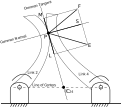
\includegraphics[width=0.60\linewidth]{fig/kennedy_sliding}
   \caption{Create a graphic similar to that found in the text for Kennedy's Theorem. Use the phrasing "figure adapted from \cite{ref:kinematics_and_dynamics}"}
   \label{fig:kennedy_sliding}
\end{figure}

\begin{figure}[!b]
   \centering
   \includegraphics[width=0.60\linewidth]{fig/single_frames}
   \caption{Create a graphic of the frames used to generate the profiles}
   \label{fig:single_frames}
\end{figure}

Before the equations are defined, a number of parameters necessary for design must be established. The eccentric distance is denoted as \textit{E}, the roller housing diameter is defined as \textit{Rr}, the radius from the fixed frame center to the center of the housing roller is defined as \textit{R}, the output pin diameter is denoted as \textit{R\textsubscript{ro}}, the radius from the fixed frame center to the output roller center is \textit{R\textsubscript{ro}}, the number of housing pins \textit{N\subscript{1}}, the number of lobes \textit{N\textsubscript{lobe}} which is generally 
\begin{equation}
N_{lobe} = N_1 - 1
\end{equation}
(however, designs with two and three lobe differences have been analyzed in \cite{ref:hsieh_traditional} and the number of output pins \textit{No}. The variable parameters during motion that are also used for calculations are the motor input angle \textit{\textphi\textsubscript{2}} and the cycloid plate rotation \textit{\textphi\textsubscript{3}}. These design parameter decisions and restrictions will be discussed further in section \ref{ch:design:single}. 

With these defined parameters, the equations necessary for generating the profiles can be developed.
Fig \ref{fig:single_frames} shows an illustration of the frames necessary for a single stage cycloid. In this case, the first link is the ground link, the second link is the motor input via the eccentric arm, and the third link is the cycloid plate itself. The interaction that must satisfy Kennedy's Theorem is between the cycloid link and the ground link, (links 1 and 3). The interaction between those two links must have an instant center that falls on the line of instant centers I\textsubscript{12} and I\textsubscript{23} that is normal to the common tangent. To create the cycloid plate profile, the location of this point must be put into the frame of the cycloid plate. Three frames are denoted in \ref{fig:single_frame}, the fixed frame \textit{F}, the motor frame \textit{M}, and the cycloid plate \textit{C}. 

\begin{figure}[!b]
   \centering
   \includegraphics[width=0.60\linewidth]{fig/single_angles}
   \caption{Create a graphic for the angles and definitions that are used to calculate}
   \label{fig:single_angles}
\end{figure}

The transforms between the fixed frame and the motor frame (Eq \ref{eq:T_fm}) and the motor frame and the cyloid frame (Eq \ref{eq:T_mc}) are first defined. 

\begin{equation} \label{eq:T_fm}
T_f^m = \left[{\begin{array}{cccc}
		cos(\phi_2) & -sin(\phi_2) & 0 & 0\\
		sin(\phi_2) & cos(\phi_2) & 0 & 0\\
		0 & 0 & 1 & 0\\
		0 & 0 & 0 & 1 \end{array} } \right]
\end{equation}

\begin{equation} \label{eq:T_mc}
T_m^c = \left[{\begin{array}{cccc}
		cos(\phi_2 - \phi_3) & -sin(\phi_2 - \phi_3) & 0 & E\\
		sin(\phi_2 - \phi_3) & cos(\phi_2 - \phi_3) & 0 & 0\\
		0 & 0 & 1 & 0\\
		0 & 0 & 0 & 1 \end{array} } \right]
\end{equation}

Next, the point point P of intersection between links 1 (the ground via the housing roller) and link 3 (the cycloid plate) can be defined using the diagram \ref{fig:single_angles}. The line between the two centers of rotation for the motor (link 1 to link 2) and the cycloid plate (link 2 to link 3) is extended. A line is then drawn from the center of the housing roller to the intersection of the extended line of centers. This defines the common normal line to the common tangent of interaction between the housing roller and the cycloid plate. Therefore, triangles can be drawn and using this definition, the angle \textpsi can be found 

\begin{equation} \label{eq:psi}
\psi = \taninv\frac{\sininv\phi_2}{\frac{R}{EN} - \cos{\phi_2}}
\end{equation}

and the location of point P with respect to the fixed frame can then be defined as 

\begin{equation} \label{eq:Cf}
C_f = \left[\begin{array}{c}
		R-Rr*cos(\psi)\\
		Rr*sin(\psi)\\
		0\\
		1
		\end{array} \right]
\end{equation}

Using these geometrically defined values based off of Kennedy's Theorem, the location of the interaction point between the cycloid plate and the roller (\textit{C\textsubscript{c}}) can be found by transforming from the fixed frame to the cycloid frame (eq \ref{eq:T_fc}) via inversion of the transformation matrices from the fixed frame to the cycloid frame (eq \ref{eq:T_cf}) multiplied by the location of the point in the fixed frame (eq \ref{eq:Cc}). This fully defines the profile of the cycloid as a function of the motor input angle \textphi\textsubscript{2} (eq \ref{eq:single_profile}).

\begin{equation} \label{eq:T_fc}
T_f^c = T_f^m * T_m^c 
\end{equation}
\begin{equation} \label{eq:T_cf}
T_c^f = \inv{T_f^c}
\end{equation}
\begin{equation} \label{eq:Cc}
C_c = T_c^f * C_o
\end{equation}

\begin{equation} \label{eq:single_profile}
C_c = \left[\begin{array}{c}
		R\cos(\frac{\phi_2}{N_1 -1}) - Rr\cos(\frac{\phi_2 + \psi(1-N_1)}{N_1-1}) - E\cos(\frac{N_1\phi_2}{N_1-1})\\
		R\sin(\frac{\phi_2}{N_1 -1}) - Rr\sin(\frac{\phi_2 + \psi(1-N_1)}{N_1-1}) - E\sin(\frac{N_1\phi_2}{N_1-1})\\
		0\\
		1
		\end{array} \right]
\end{equation}

These equations fully define the basic cycloidal plate profile. However, real life is generally not as friendly to these perfect equations. Therefore, design considerations must be taken into account when actually manufacturing the wobble plates. These undersizing considerations for machine tolerances are well developed in \cite{ref:design_and_application} and the recommended undersizing is applied to the design of the cycloids tested in this work. Finally, equations to determine whether undercutting exists in the cycloid profile are presented in \cite{ref:ye} to aid in sizing of the cycloidal profile. 



\section{Single Stage Design} \label{ch:design:single}
% Talk about items that are specific to a single stage design, specifically the load calculations and such to size the plates and the disks 

After the development of the basic equations for the profile of the cycloid, the practical design considerations must take place to allow for the desired loads and reduction to be carried through the cycloid for the given application. These application specific design values will be discussed briefly as they pertain to the literature. This actuator was originally designed by NASA robotics engineers at NASA: Johnson Space Center. The design equations used are presented to lay the foundation for the analysis and the testing results contributed by this Thesis.

\subsection{Single Stage Cycloid Design Requirements}

\begin{table*}[!b]
  \vskip0.2cm
  \caption{Designed Duty Cycles for System}
  \label{duty_cycle}
  \begin{center}
    \vskip-0.2cm
    \begin{tabular}{|p{0.10\textwidth}||p{0.15\textwidth}||p{0.15\textwidth}| |p{0.15\textwidth}| |p{0.15\textwidth}|}
    \hline
    Time Used & Output Torque (Nm) & Output Speed (RPM) & Actuator Torque (Nm) & Actuator Speed (RPM)\\
    \hline
    5\% & 2440 & 6.8 & 554.7 & 33.9\\
    \hline
    20\% & 1627 & 6.8 & 369.8 & 33.9\\
    \hline
    60\% & 542 & 15.3 & 123.3 & 76.3\\
    \hline
    15\% & 135 & 15.3 & 30.8 & 76.3\\
    \hline
    \end{tabular}
  \end{center}
\end{table*}

In 2007 and 2008, NASA developed a manned rover prototype for planetary surfaces for future missions \cite{ref:rover}.
This robotic vehicle is made up of six independent wheel modules, each with their own drive, steering, and both active and passive suspension.
In 2014, a new prototype wheel module was designed and created to analyze potential technologies that could be used in these applications.
In the new design layout, it was possible for the drive wheels to counter-rotate against the steering and put large shock loads into the steering system.
These requirements called for a compact package, high load, high shock load, and allowed tolerance of backlash lent themselves to the selection of a cycloidal drive for the steering actuator.
The prototype wheel module layout can be seen in Fig \ref{fig:wheel_module}.

\begin{figure}[t]
   \centering
   \includegraphics[width=0.40\linewidth]{fig/wheel_module_CAD}
   \caption{CAD model of rover wheel module prototype.
   Suspension arms hold the steering column.
   Each wheel has an in-wheel drive motor.}
   \label{fig:wheel_module}
\end{figure}

Based on the load cases, the actuator was required to output a stall torque of 2,440 Nm (1800 ft-lb) with a max output speed of 1.57 rad/s (90 deg/s) at 1,626 Nm (1200 ft-lb).
The required torque/speed data points are presented in Table \ref{duty_cycle} with an assumed loss of 88\% chosen based on the available literature.
The actuator layout for the vehicle placed the motor and cycloid off center of the steering axis with an additional 5:1 reduction into the steering column, thus decreasing the torque needed for the cycloid output, but increasing the potential shock loading.

\subsection{Force Analysis and Sizing} \label{ch:design:single:force_analysis}

First, the motor and cycloid reduction were sized together to determine the appropriate motor and reduction to use for the system. The motor selected was a Parker Frameless Kit Motor, model K089200-7Y with no hall commutation with a cycloid reduction of 59:1 before going into an additional 5:1 reduction to the final steering output. The motor is commutated using a Renishaw RM-44 magnetic encoder mounted to the input shaft. 

Knowing the reduction must be 59:1 and the output torque of the cycloid before the final 5:1 redution, the maximum load developed by the cycloid (\textit{F\textsubscript{max}}) is 488 Nm and the maximum speed of the cycloid {\textomega\textsubscript{max}} is 7.85 rad/s. These values can be used in conjunction with a well defined set of equations presented in previous works \cite{ref:malhorta}, \cite{ref:li}, and \cite{ref:unified_approach} to determine the allowable sizes of the components of the system. The analysis presented by Malhorta and Parameswaran details the analysis necessary for the loads on the housing pins and the output pins for a single stage degisn. This methodology has been adopted for this work and will be further expanded upon in Chapter \ref{ch:dual} so it is presented in its completeness here. 

\begin{figure}[t]
   \centering
   \includegraphics[width=0.40\linewidth]{fig/single_stage_loads}
   \caption{TODO - Make a figure with the loads drawn out for a single stage design}
   \label{fig:single_loads}
\end{figure}

The interaction between the elements of a single stage cycloid can be seen in Fig. \ref{fig:single_loads} that details the forces present in a cycloid. The input force from the motor drives through the eccentric bearing to the wobble plate. These loads are then reacted through the housing rollers and output pins. One will notice that the loads can only form on one half of the rollers and pins at a time, as these members are in compression, and if a tension force forms, they will separate and not carry load. In a perfectly manufactured arrangement, the number of lobes in contact, \textit{N\textsubscript{lc}} and output pins in contact, \textit{N\textsubscript{oc}}, is simply 

\begin{equation}
N_{lo} = \frac{N_{lobes}}{2},\ if\ N_{lobes}\ is\ even 
\end{equation}
\begin{equation}
= \frac{N_{lobes} - 1}{2},\ if\ N_{lobes}\ is\ odd 
\end{equation}
\begin{equation}
N_{oc} = \frac{N_{pins}}{2},\ if\ N_{pins}\ is\ even 
\end{equation}
\begin{equation}
= \frac{N_{pins} - 1}{2},\ if\ N_{pins}\ is\ odd 
\end{equation}

There are a geometric number of values depicted in Fig. \ref{fig:single_loads} that must be defined in order to successfully calculate the loads in the next step. These are written simply in \cite{hwang_geometry} and are shown below in equations [\ref{eq:single_b} -- \ref{eq:single_l}]. 

\begin{equation} \label{eq:single_b}
\beta_i = \frac{2\pi i}{N_1}
\end{equation}
\begin{equation} \label{eq:single_d}
d = \sqrt{\rho_1^2 + R^2 - 2 \rho_1 R \cos{\beta_i}}
\end{equation}
\begin{equation} \label{eq:single_alpha}
\alpha_i = \sin^{-1}\left[{\frac{R \sin{\beta_i}}{d}}\right]
\end{equation}
\begin{equation} \label{eq:single_rho2}
\rho_2 = \rho_1 - E
\end{equation}
\begin{equation} \label{eq:single_l}
l_i = \rho_2 \sin{\alpha_i}
\end{equation}

Using this knowledge, the forces on the contacting lobes and pins can be calculated. This calculation methodology starts with a power analysis to determine the forces on the output pins (eq. \ref{eq:single_power}). Using this as a basis, equations for the forces in the x-direction (eq \ref{eq:single_x}), y-direction (eq. \ref{eq:single_y}), and the moment about the wobble-plate's center (eq. \ref{eq:single_torque}) can be written for any reducer with \textit{N\textsubscript{c1}} lobes (\texit{N\textsubscript{1}} housing rollers) and \textit{N\textsubscript{p1}} output pins. The forces on housing roller \textit{i} is denoted as \textit{F\textsubscript{ri}} and on output pin \textit{j} as \textit{F\textsubscript{oj}}.

\begin{equation} \label{eq:single_power}
M_a = \frac{R_o}{N_1} \sum_{j=1}^{N_{oc}} F_{oj} \sin(\beta_j + N_1 \phi_2)
\end{equation}
\begin{equation} \label{eq:single_input}
Ma = F_{input} E \cos(N_1 \phi_2 + \gamma)
\end{equation}
\begin{equation} \label{eq:single_x}
\sum_{i=1}^{N_{lc}} F_{ri} \cos{\alpha_i} - \sum_{j=1}^{N_{oc}} F_{oj} \cos(N_1*\phi_2) - F_{input} \sin{\gamma} = 0
\end{equation}
\begin{equation} \label{eq:single_y}
-\sum_{i=1}^{N_{lc}} F_{ri} sin{\alpha_i} + \sum_{j=1}^{N_{oc}} F_{oj} sin(N_1*\phi_2) + F_{input} \cos{\gamma} = 0
\end{equation}
\begin{equation} \label{eq:single_torqe}
\sum_{i=1}^{N_{lc}}F_{ri} l_i - \sum_{j=1}^{N_{oc}}F_{oj} R_o \sin(\beta_j + N_1 \phi_2) = 0
\end{equation}

In order to solve this system of equations, an additional assumption must be made. That is, that the forces on the pins and rollers are relative to their length \textit{l\textsubscript{ij}}, that is 

\begin{equation} 
\frac{F_{1i}}{l_{1i}} = constant 
\end{equation}
\begin{equation}
\frac{F_{oi}}{l_{oi}} = constant
\end{equation}

Using this system of equations, the forces on the input pins can be determined for a given cycloid system. However, these equations assume that the forces are being shared perfectly across all lobes and pins that could be in contact at any given time. Due to the nature of real life and manufacturing tolerances, fewer than the ideal number of pins will be in contact. Therefore, the pins should be sized such that if a single pin takes this force, it will not fail, and it can be assumed that the plate would deform such that additional pins and lobes would begin to take the load. Using these assumptions, the maximum loads on a single lobe and output roller for the designed cycloid are shown in Table \ref{table:single_loads} which leads to the necessary sizing of components in Table \ref{table:single_sizing}.

\begin{table}
  \vskip0.2cm
  \caption{Single Stage Calculated Loads}
  \label{table:single_loads}
  \begin{center}
    \vskip-0.2cm
    \begin{tabular}{|c|c|}
    \hline
	Variable & Value\\
	\hline
	\textit{F\textsubscript{roller}} & 11 kN\\
	\hline
	\textit{\textsigma\textsubscript{roller}} & 643 kPa\\
	\hline
	\textit{F\textsubscript{output-pin}} & 14.8 kN\\
	\hline
	\textit{\textsigma\textsubscript{output-pin}} & 722 kPa\\
	\hline
    \end{tabular}
  \end{center}
\end{table}

\begin{table}
  \vskip0.2cm
  \caption{Single Stage Design Values}
  \label{table:single_sizing}
  \begin{center}
    \vskip-0.2cm
    \begin{tabular}{|c|c|}
    \hline
	Design Variable & Value\\
	\hline
	\textit{N\textsubscript{lobes}} & 59\\
	\hline
	\textit{N\textsubscript{rollers}} & 60\\
	\hline
	\textit{Eccentricity} & 0.762 mm\\
	\hline
	\textit{Roller Offset Radius} & 50.8 mm\\
	\hline
	\textit{Housing Roller Radius} & 1.58 mm\\
	\hline
	\textit{Cycloid Plate Thickness} & 7.94 mm\\
	\hline
	\textit{Cycloid Plate Material} & 17-4 PH Stainless Steel\\
	\hline
	\textit{Housing Roller Material} & Stainless Steel \todo{verify}\\
	\hline
	\textit{Output Pin Material} & Stainless Steel \todo{verify}\\
	\hline
    \end{tabular}
  \end{center}
\end{table}

\subsection{Final Single Stage Design} \label{ch:design:single:final}

Using the equations and analysis laid out in Section \ref{ch:design:basic_calc:overview} and Section \ref{ch:design:single:force_analysis}, the final design was completed and manufacutred. In the design, the wobble-plates need a thickness of 7.94 mm, to accomplish this thickness and balance the system for vibrations, three wobble-plates are used in tandem, each 120\textdegree offset from the other. In this design, the housing rollers are free to rotate. A channel is cut into the housing and the pin rests in that channel, so it is assumed they will slide freely. The output pins however are pressed into the output plate, so they are assumed to remain fixed through operation, and this assumption is validated in the results. The cross section profile of the CAD model can be see in Fig \ref{fig:single_stage} and an image of the actual system can be seen in Fig \ref{fig:single_stage_actual}.

\begin{figure}
   \centering
   \includegraphics[width=0.5\linewidth]{fig/exploded_labeled}
   \caption{Exploded view of the cycloidal reducer.
   Three wobble plates are driven by the input shaft with 120\textdegree\ offsets.
   The ring pins are are free pins inserted in the housing.
   The output has pins run through all three wobble plates to harness the counter-rotation for the drive output.}
   \label{fig:single_stage}
\end{figure}

\begin{figure}
   \centering
   \includegraphics[width=0.5\linewidth]{fig/single_stage_actual}
   \caption{Get a picture of the actual assembly to put here}
   \label{fig:single_stage_actual}
\end{figure}


\section{Housing Pin Motion Analysis} \label{ch:design:pin_roll_1s}
% Talk about the rolling of the housing pins in a single stage. The trick here is to try to say "this is new, pay attention." Also, skirt around the output pins, haven't done that part and that's okay.

Through testing and analysis, a gap in the literature was identified pertaining to the relative sliding between the cycloid plate and the housing pins. The cycloid profile is generated based off of Kennedy's Theorem about links in contact and their required instant centers, discussed in Section \ref{ch:design:basic_calc:overview}. Kennedy's Theorem states that for two links to have only sliding motion with respect to each other, the point of contact must lie along the line of centers between each links instant center shown in \ref{fig:kennedy_rolling}, otherwise, sliding must occur. Using this fact, equations for the necessary sliding motion between the cycloid plate and the rollers needs to be developed to make a more accurate predictive loss model for the compact cycloid designs.

\begin{figure}[!b]
   \centering
   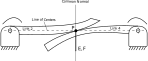
\includegraphics[width=0.7\linewidth]{fig/kennedy_rolling}
   \caption{Create a picture of the rolling contact for kennedy theorem}
   \label{fig:kennedy_rolling}
\end{figure}

\subsection{Sliding Equations} \label{ch:design:pin_roll_1s:sliding_equations}

Kennedy's Theorem states that the two links in contact can only move in the direction of the common normal and rotate about the instant center between the two links. In Fig \ref{fig:kennedy_sliding} different velocities can be defined. First, the point of contact, P, that is shared on each link can only have a velocity in the \textit{S} direction, along the common nomral to maintain contact. Then, velocities \textit{M} and \textit{L} can be defined as the velocities normal to \textit{S} for link 1 and link 2 respectively. The difference between \textit{M} and \textit{L} is the sliding velocity between the two links \cite{ref:kinematics_and_dynamics}.

Using these definitions, the relationship between \texit{M} and \textit{L} can be derived for a single stage cycloid. In this case, there is no motion of the point along the common normal between the two links in contact, the cycloid plate and the housing roller, because the housing roller is fixed in space. Therefore, the only relative velocity between the two links comes with the rotation about the instant center between the cyloid plate and housing roller. This can be calculated simply using the length from the instant center to the contact point, \textit{l\textsubscript{c}} and the rotational velocity of the cycloid plate, \textit{\textomega\textsubscript{3}} for each pin around the housing. 

\begin{equation} \label{eq:single_slide_offset}
offset = i \frac{2\pi}{N_1}
\end{equation}
\begin{equation} \label{eq:single_slide_length}
l_{ci} = \sqrt{\left[R-R_r\cos\psi - E N_1 \cos(\phi_2 - offset)\right]^2 
+ \left[-R_r \sin{\psi} + E N_1 \sin(\phi_2 - offset)\right]^2 }
\end{equation}
\begin{equation} \label{eq:single_slide_vel}
V_i = \omega_3 * l_{ci}
\end{equation}

Using this relationship, the sliding velocity between the cycloid plate and housing rollers can be determined. However, the cycloid is designed such that the pins rest in the housing and are free to rotate, therefore, the sliding velocity will be translated to a rotational velocity of the pin. An example of the relative sliding velocities for four different input angles \textphi\textsubscript{2} can be seen in Fig \ref{fig:single_sliding} with an input velocity \textomege\textsubscript{2} of 1.5 rad/s.

\begin{figure}[!b]
   \centering
   \begin{tabular}{cc}
	   \includegraphics[width=0.48\linewidth]{fig/single_vel_0pi} &
	   \includegraphics[width=0.48\linewidth]{fig/single_vel_pi_2} \\
	   \includegraphics[width=0.48\linewidth]{fig/single_vel_pi} &
	   \includegraphics[width=0.48\linewidth]{fig/single_vel_3pi2}
   \end{tabular}
   \caption{The linear velocity at the edge of each pin in the single stage cycloid through one input rotation}
   \label{fig:single_sliding}
\end{figure}

\subsection{Predicted Single Stage Roller Losses} \label{ch:design:pin_roll_1s:predicted_losses}

Due to the assertion that there is sliding of some type (either the plate along the pin, or the pin rolling in the housing) and there are forces acting on these pins shown in Fig \ref{fig:single_force}, there is some loss associated with this interaction that has not previously been captured in the literature. Using the forces developed along the pins in Section \ref{ch:design:single:force_analysis} and the sliding velocities for each pin developed in Section \ref{ch:design:pin_roll_1s:sliding_equations}, the power losses for the system can be estimated using 

\begin{equation} \label{eq:single_power_loss}
P_L = \sum_{i=1}^{N_{lc}}\mu F_ri V

Note that there will only be losses on pins that have a contact force, which was defined as the number of pins divided by two at any given time. The estimated losses due to the cycloid disk rolling along the housing pins, which must then slide in the housing can be calculated for the single stage cycloid for a given range of inputs. These results are shown in Table \ref{table:single_slide_estimate}.

\begin{figure}[!b]
   \centering
   \begin{tabular}{cc}
	   \includegraphics[width=0.48\linewidth]{fig/single_force_0} &
	   \includegraphics[width=0.48\linewidth]{fig/single_force_pi_2} \\
	   \includegraphics[width=0.48\linewidth]{fig/single_force_pi} &
	   \includegraphics[width=0.48\linewidth]{fig/single_force_3pi2}
   \end{tabular}
   \caption{The forces on each of the pins in the single stage cycloid through one rotation}
   \label{fig:single_sliding}
\end{figure}

\begin{figure}[!b]
   \centering
   \begin{tabular}{cc}
	   \includegraphics[width=0.48\linewidth]{fig/single_power_0} &
	   \includegraphics[width=0.48\linewidth]{fig/single_power_pi2} \\
	   \includegraphics[width=0.48\linewidth]{fig/single_power_pi} &
	   \includegraphics[width=0.48\linewidth]{fig/single_power_3pi2}
   \end{tabular}
   \caption{The losses contributed by the interation with each housing roller in the single stage cycloid through a single rotation.}
   \label{fig:single_sliding}
\end{figure}

\todo[inline]{Make a table of losses for the single stage slidnig} 

The losses of each pin can be summed to get the instantanous power loss of the cycloid due to the interaction between the cycloid plate and the housing pins. For this case the desired output is 1.5 rad/s and 94 Nm. If a coefficient of sliding friction (\textmu) is assumed to be 0.1, the losses associated solely with this interaction are 19.62 W, resulting in an effciency of 87.8\% due only to the sliding at this interface. This number is heavily dependant on \textmu, if \textmu decreases to 0.5, the efficiency increases to 93.5\%, \textmu increased to 2.0, the efficiency decreases to 78\%.Therefore, the optimization of this interaction is pivotal. Nearly all manufacturers of cycloidal drives use roller bearings at this interaction, which have \textmu of 0.01 or less, resulting in efficiencies of 98.6\% or higher. So when designing a compact cycloid for a robotic application, great care must be taken in designing the surfaces and sliding of this interface. 
%!TEX root = thesis_main.tex

\chapter{Testing and Analysis of single-stage Cycloid}\label{ch:single}
%Give and Overview of Chapter 3

There is a gap in the literature for the in-use efficiency and lifetime characteristics of cycloidal reducers of the compact design that was presented in Chapter \ref{ch:design_1s}. Previously, the longest set of test data for a compact cycloid was 80 minutes. This work aims to develop an understanding of the in-use characteristics of the single-stage compact design cycloid reducer in both efficiency and the initial analysis of lifetime for a cycloid of this type. Therefore, the single-stage design previously discussed was run through a long duration life-cycle with efficiency testing performed periodically to understand these pertinent characteristics. The actuator was run for over 300 hours with 130k output revolutions. The peak efficiency achieved through this time was 81\% which shows this actuator is competitive in efficiency with a harmonic drive. In addition, no appreciable degradation of performance was seen from break in until testing completion, showing the actuator's lifetime easily exceeds the current testing time.  

This work has been submitted to the International Conference on Robotics and Automation, ICRA with the title ``Cycloidal Geartrain In-Use Efficiency Study.'' Portions of this section are taken directly from this publication. This chapter will first cover the experimental test setup in Section \ref{ch:single:test_setup}. The results of this testing are presented in Section \ref{ch:single:eff_results}. An analysis of the wear of the components is presented in Section \ref{ch:single:wear_analysis}. Finally, a discussion of these results is given in Section \ref{ch:single:discussion}.

\section{Test Setup} \label{ch:single:test_setup}
%Give the test setup for the single-stage, basically pull the info from the paper 

The intent of testing the cycloidal drive is to experimentally determine and compare the in-use efficiency results to the published performance data for a comparable harmonic drive.
To accomplish this, the actuator was mounted to a Futek TF600 5000inlb load cell to measure output torque of the actuator.
The load cell signal was collected through a analog to digital converter and converted to standard units on the motor driver.
A verification of torque readings was completed using a calibrated torque wrench to ensure accuracy of the conversion.
Load was regulated by a Magtrol HB-1750 hysteresis brake.
A 36:1 speed increase was added via three chain stages between the output of the actuator and the hysteresis brake to achieve the desired applied loads.
The hysteresis brake was powered using a separate 24V Lambda-TDK power supply that was controlled through a RS-485 communication link to the test computer.
NASA's 'turbodriver' motor driver was used for commanding motor currents.
The motor driver was powered by a TDK-Lambda 12V supply for logic power and a TDK-Lambda 150V and 5A supply for high voltage power.
A hysteresis current controller was used on the motor drive to accurately provide torque producing current to the motor.
The motor driver monitored the actuator power by measuring torque from the load cell and speed with an incremental encoder located at the actuator motor shaft.
The test computer monitored the high voltage supply and recorded voltage and current to determine input power to the system and received data from the motor driver to calculate output power.
The test setup is shown in Fig \ref{fig:test_setup}.

\begin{figure}[t]
   \centering
   \includegraphics[width=0.75\linewidth]{fig/test_stand}
   \caption{Experimental Test Setup.
   The cycloid actuator is mounted to structure via the load cell.
   There is a speed increase so the brake can generate enough torque on the system.
   Not pictured is the controlling computer, motor driver, and high voltage supply.}
   \label{fig:test_setup}
\end{figure}

Due to the tightly integrated actuator design, the motor and cycloid cannot be separated to purely isolate the losses in the cycloid.
The efficiency map of the motor over its torque and speed range was provided by Parker Motors.
For calculation purposes, this table is used as a lookup table for efficiency of the motor given the current motor velocity and rms input current.
While this does generate a level of uncertainty in the data, these motors are mass manufactured and defects are assumed to be small.
The error in the motor efficiency map is assumed to be small and would not influence the perceived trends and results.
Power losses in the motor driver were also taken into consideration by calculating power losses in the IGBT that drives the motor.
Instantaneous current draw and a switching frequency of 12 kHz were used for the calculation, neglecting small leakage losses \cite{ref:IGBTPower}.

\begin{figure}[t]
   \centering
   \includegraphics[width=\linewidth]{fig/eff_test_profile_v4}
   \caption{Testing profile for efficiency.
   At each speed step, torque is ramped up through five different levels, then the speed is increased.
   At the last step, the maximum of the supply was reached so motor velocity dropped.}
   \label{fig:eff_profile}
\end{figure}

The system was tested in two separate ways, an efficiency cycle and a long term drive cycle.
The efficiency cycle was run multiple times throughout the lifetime testing, first after the actuator achieved steady state efficiency, and again after each 100 hours of testing.
For the efficiency cycle, the actuator is subjected to eight velocity steps increasing 0.25 rad/s each time.
In each velocity step, the torque is ramped up and maintained for 15 seconds at values of 1Nm, 15Nm, 52Nm, 94Nm, and 189Nm.
This testing profile can be seen in Fig \ref{fig:eff_profile}.
The long term drive cycle was run continuously each day for 6 to 12 hours with the duty cycles shown in Table \ref{table:long_run}.
The total runtime of the system, not including the initial checkout and verification of the actuator, has been 303 hours.

\begin{table}[t]
  \vskip0.2cm
  \caption{Long Run Drive Cycle}
  \label{table:long_run}
  \begin{center}
    \vskip-0.2cm
    \begin{tabular}{|c||c||c|}
    \hline
    Time (s) & Velocity (rad/s) & Torque (Nm)\\
    \hline
    150 & 1.0 & 0.0\\
    \hline
    150 & -1.0 & 0.0\\
    \hline
    60 & 0.5 & 26.0\\
    \hline
    60 & -0.5 & 26.0\\
    \hline
    150 & 1.5 & 10.0\\
    \hline
    150 & -1.5 & 10.0\\
    \hline
    30 & 1.0 & 50.0\\
    \hline
    30 & -1.0 & 50.0\\
    \hline
    300 & 0.5 & 18.0\\
    \hline
    300 & -0.5 & 18.0\\
    \hline
    \end{tabular}
  \end{center}
\end{table}

It should be noted that the actuator was used briefly in the robot validation after initial development and construction of the prototype wheel module.
The total time of use was approximately three hours.
Afterwards, it was removed from the wheel module and subjected to the characterization that is discussed in this work.
The motor has a continuous current rating of 4.3 A\textsubscript{rms} and a peak rating of 15A\textsubscript{rms}.
The actuator was designed to be liquid cooled to allow operations above the continuous values, but this could not be achieved during testing.
For long duration testing, the torque values were decreased to avoid thermal issues.
The motor was tested to approximately 6A\textsubscript{rms} during efficiency testing due to the limit of the power supply.
Also, the motor driver's rated limits are 150V, therefore the actuator's maximum rated speeds could not be tested.
The nominal cycle of the actuator as seen in Table \ref{table:duty_cycle} is still achievable and has been tested.



\section{Results} \label{ch:single:eff_results}
%Discuss the results that we achieved 
% - burn in time 
% - efficiency over the current run time 
% - specific efficiency runs
% - compare to the "expected" efficiency from the rolling anlaysis 

Duty cycle testing was performed first on the actuator.
These tests were done at lower torques to prevent the motor from overheating to allow extended duration testing.
The total test time prior to these duty cycle tests was approximately 5.2 hours to bring up and check out the actuator testbed system.
Once this checkout was complete, the 300 hours of duty cycle testing were conducted over the course of 39 days with the drive cycle presented in Table \ref{table:long_run}.
Three of the torque/speed combinations in forward and reverse are plotted on Fig \ref{fig:long_run} to show the general characteristic trends seen in actuator performance.

\begin{figure}[!b]
   \centering
   \includegraphics[width=\linewidth]{fig/total_runtime}
   \caption{Efficiency over time for three different speed/torque profiles during the drive cycle.
   The forward motion can be seen with the dotted line, reverse with the solid line.
   Testing transitions from day to day are denoted with vertical dotted lines.
   At the onset of testing, visible efficiency gains are made.
   As each day begins, there is a clear warm-up period before steady state.
   }
   \label{fig:long_run}
\end{figure}
\todo[inline]{fix the legend to be a real size}

After the break in period and steady state performance was achieved, a profile of speeds and torques (see Fig \ref{fig:eff_profile}) were run on the actuator to show the relationship between speed, torque, and efficiency.
This profile was run three times and the results at each torque and speed combination were averaged. The first efficiency cycle was run as seen in Fig \ref{fig:eff_results}. Efficiency cycles were run after each subsequent 100 hours of testing to understand performance over time. The final efficiency test is shown in Fig \ref{fig:eff_results_final}.

\begin{figure}[h]
   \centering
   \includegraphics[width=0.8\linewidth]{fig/eff_test_bar_plot_v3}
   \caption{Efficiency of the single-stage cycloid after 100 hours of testing. Grouping of average efficiencies at each torque step.
   Efficiency depends heavily on torque, and slightly on speed.}
   \label{fig:eff_results}
\end{figure}

\begin{figure}[h]
   \centering
   \includegraphics[width=0.8\linewidth]{fig/eff_final}
   \caption{Efficiency of single-stage cycloid after 300 hours of testing. No appreciable loss of efficiency after 129k revolutions. TODO - make the legend look the same as the one above }
   \label{fig:eff_results_final}
\end{figure}
\todo[inline]{make the legend size reasonable and the same}

\section{Wear Analysis} \label{ch:single:wear_analysis}
% Look at the pictures that we took to say "check it out, this thing can probably go for a lot longer based on how well it's done so far."
% The only real thing to look at is those plastic pieces and talk about uneven wearing on the output pins. 

After completion of the 300 hours, and 129k cycles of testing, the actuator was disassembled to qualitatively analyze the wear patterns on the cycloid. This analysis gives an interesting look as to the wear and potential lifetime of the system. 

The first note is that the grease used, Red 'N Tacky from Lucas Oil, had turned a much darker color, nearly black. The system with the output pins and plate removed can be seen in Fig \ref{fig:single_full}. After removing the individual pieces and cleaning, the wear patterns in the system become clear. The cycloid plate, Fig \ref{fig:cycloid_plate}, shows smoothing of the peaks of the lobes on the plate, where they interact with the housing pins, but shows no wear deeper in the pockets. This indicates that the machining tolerances were such that these never interacted with the pins. The wear along the faces of each lobe were consistent around the profile, suggesting each lobe carried load at some point in each cycle. Additionally, the internal holes for the output pins shows relatively even wear. These results are typical for each of the three cycloid plates. 

\begin{figure}[t]
   \centering
   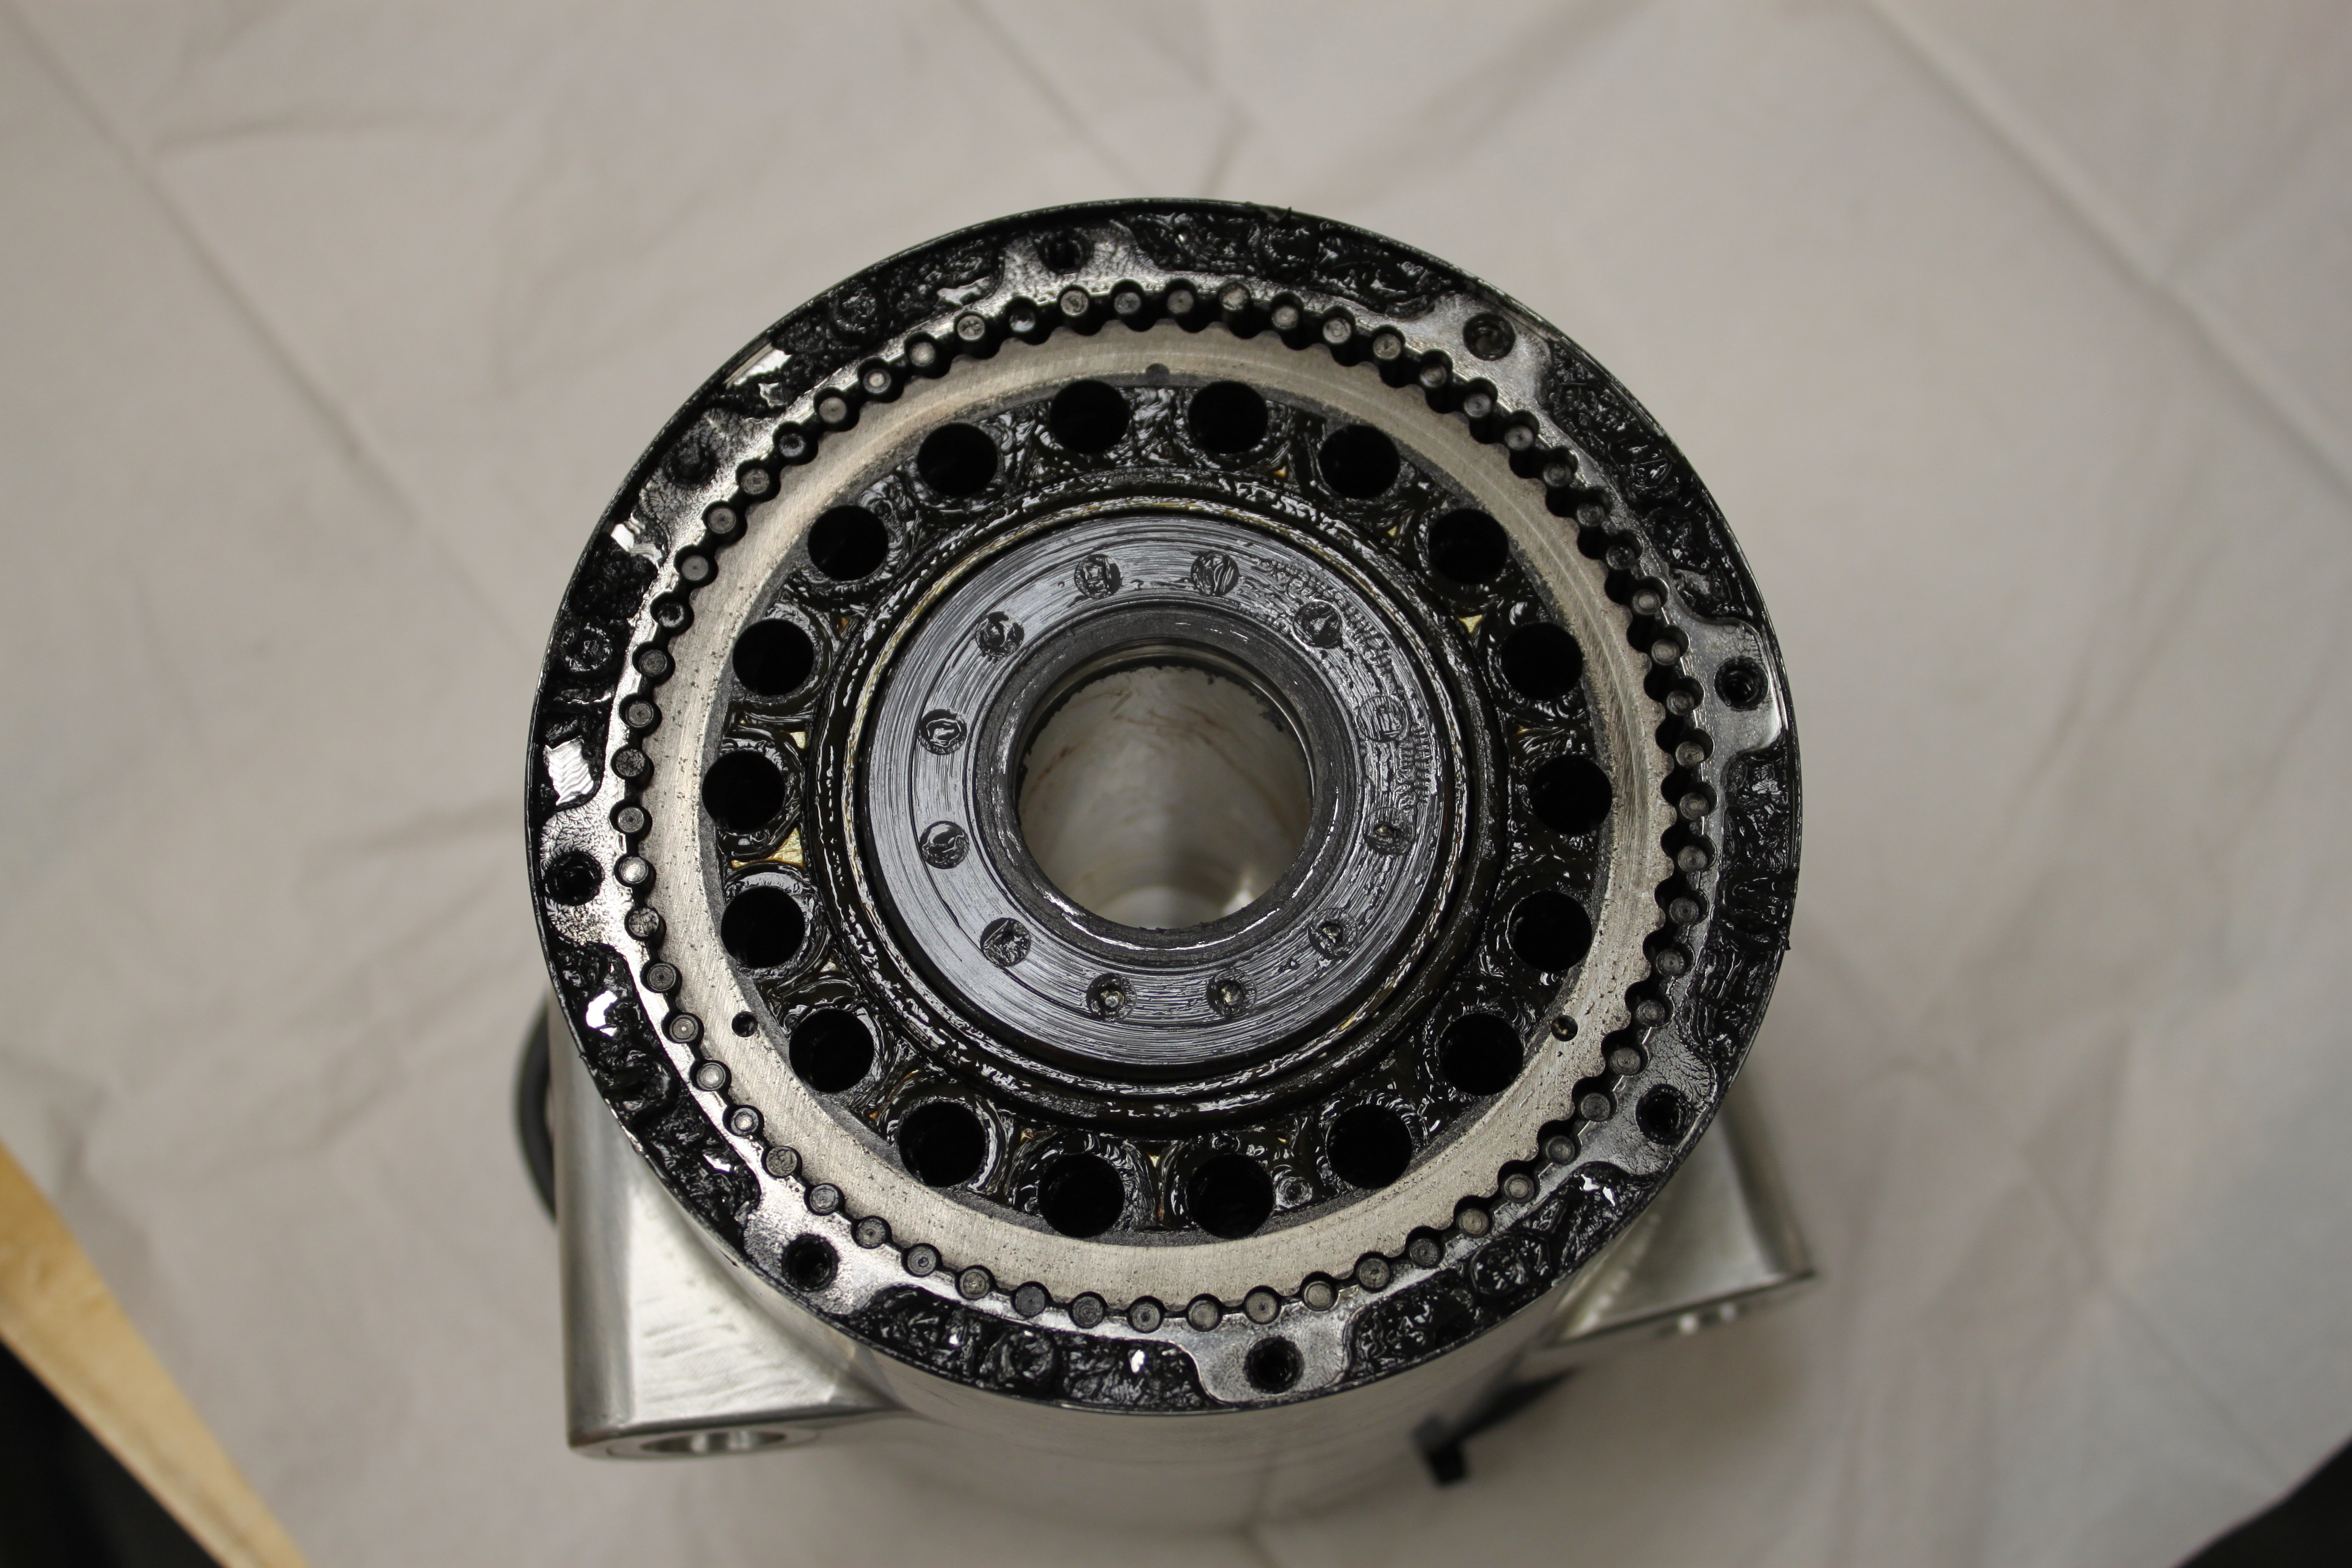
\includegraphics[width=0.4\linewidth]{fig/single_full}
   \caption{The single-stage cycloid with the output plate removed. The initially red grease has been turned nearly black through operation, likely due to metal deposits from the wearing in of the system.}
   \label{fig:single_full}
\end{figure}

\begin{figure}[!b]
   \centering
   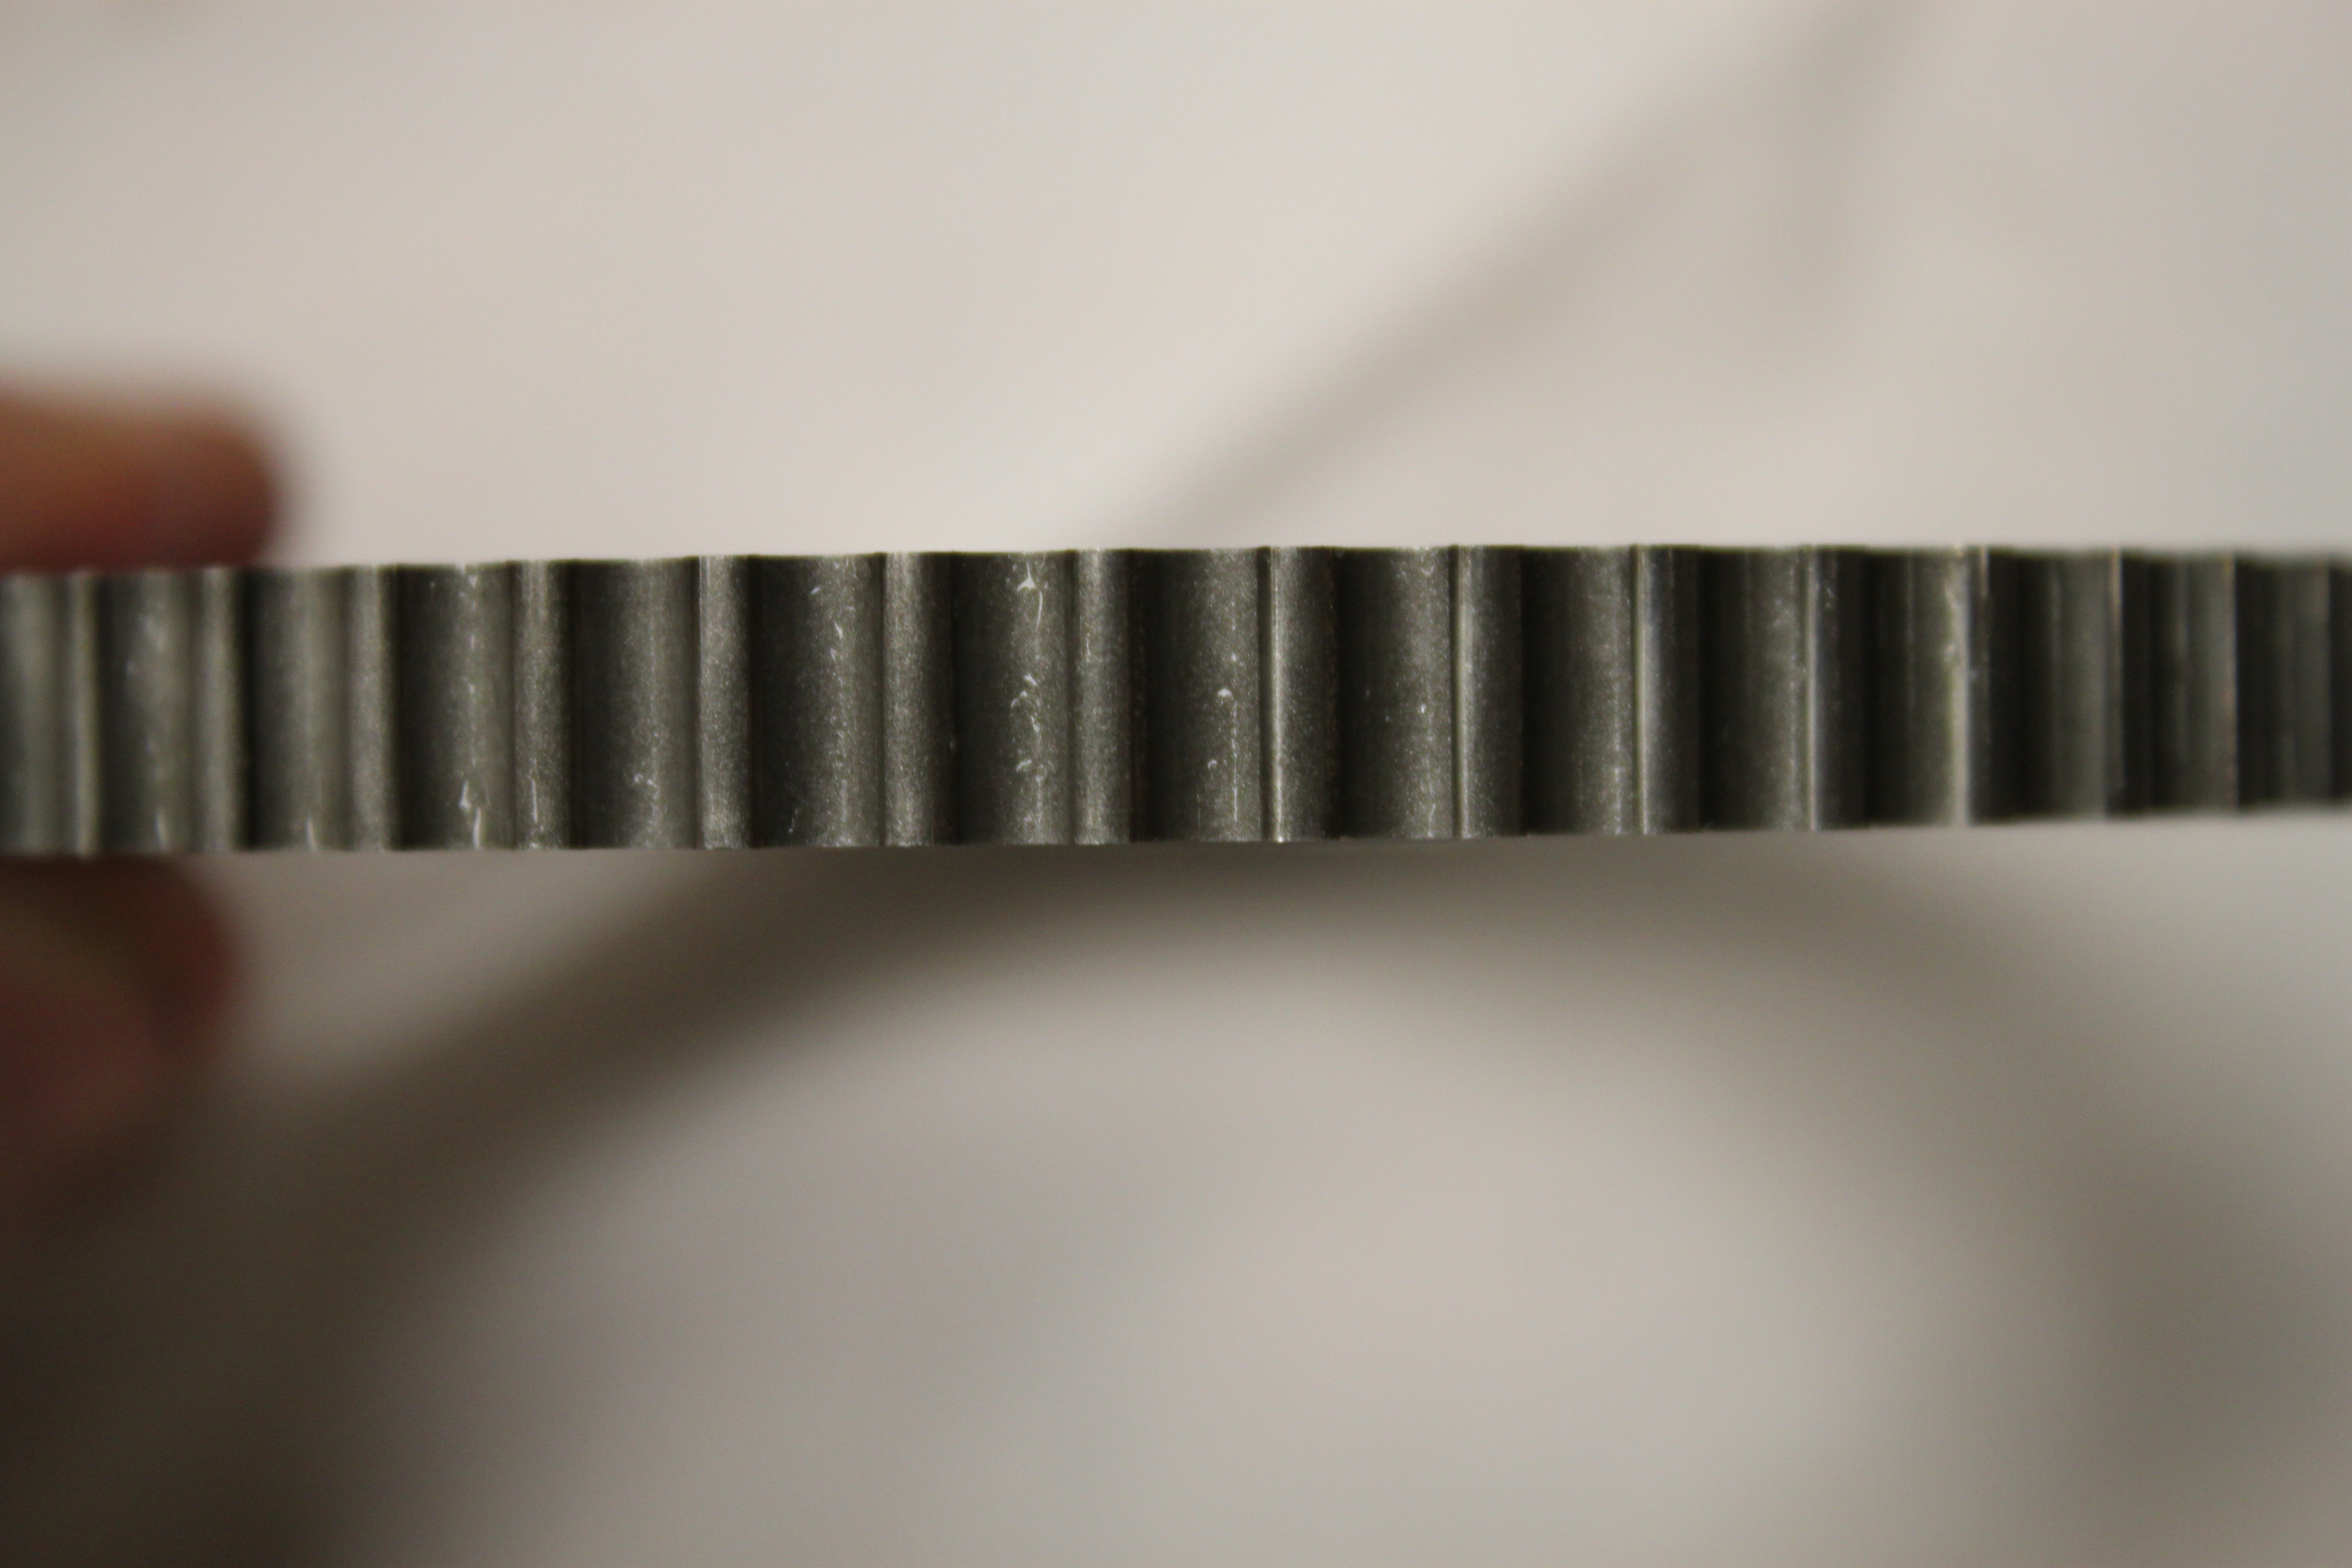
\includegraphics[width=0.8\linewidth]{fig/cycloid_plate}
   \caption{The profile of one of the cycloid plates from the single-stage actuator. Each lobe shows smoothing along convex portion of the lobe and no wear along the concave portion. The wear is also uniform around the profile, showing relatively even load distribution around the profile during operation.}
   \label{fig:cycloid_plate}
\end{figure}


Three of the housing pins can be seen as an example in Fig \ref{fig:single_housing_pins}. The wear on these pins is uniform all the way around the pin. This shows that the pin was in fact rotating in the housing during operation, as determined by the sliding analysis in Section \ref{ch:design:pin_roll_1s:sliding_equations}. These three pins are also indicative of the other 57 pins, as each had relatively uniform wear around the profile. This, coupled with the cycloid plate, suggests that during the bulk of operation, the load was shared amongst all of the lobes and pins, rather than a small set of them. This potentially could have happened during the break in period of the system as well. 

\begin{figure}[t]
   \centering
   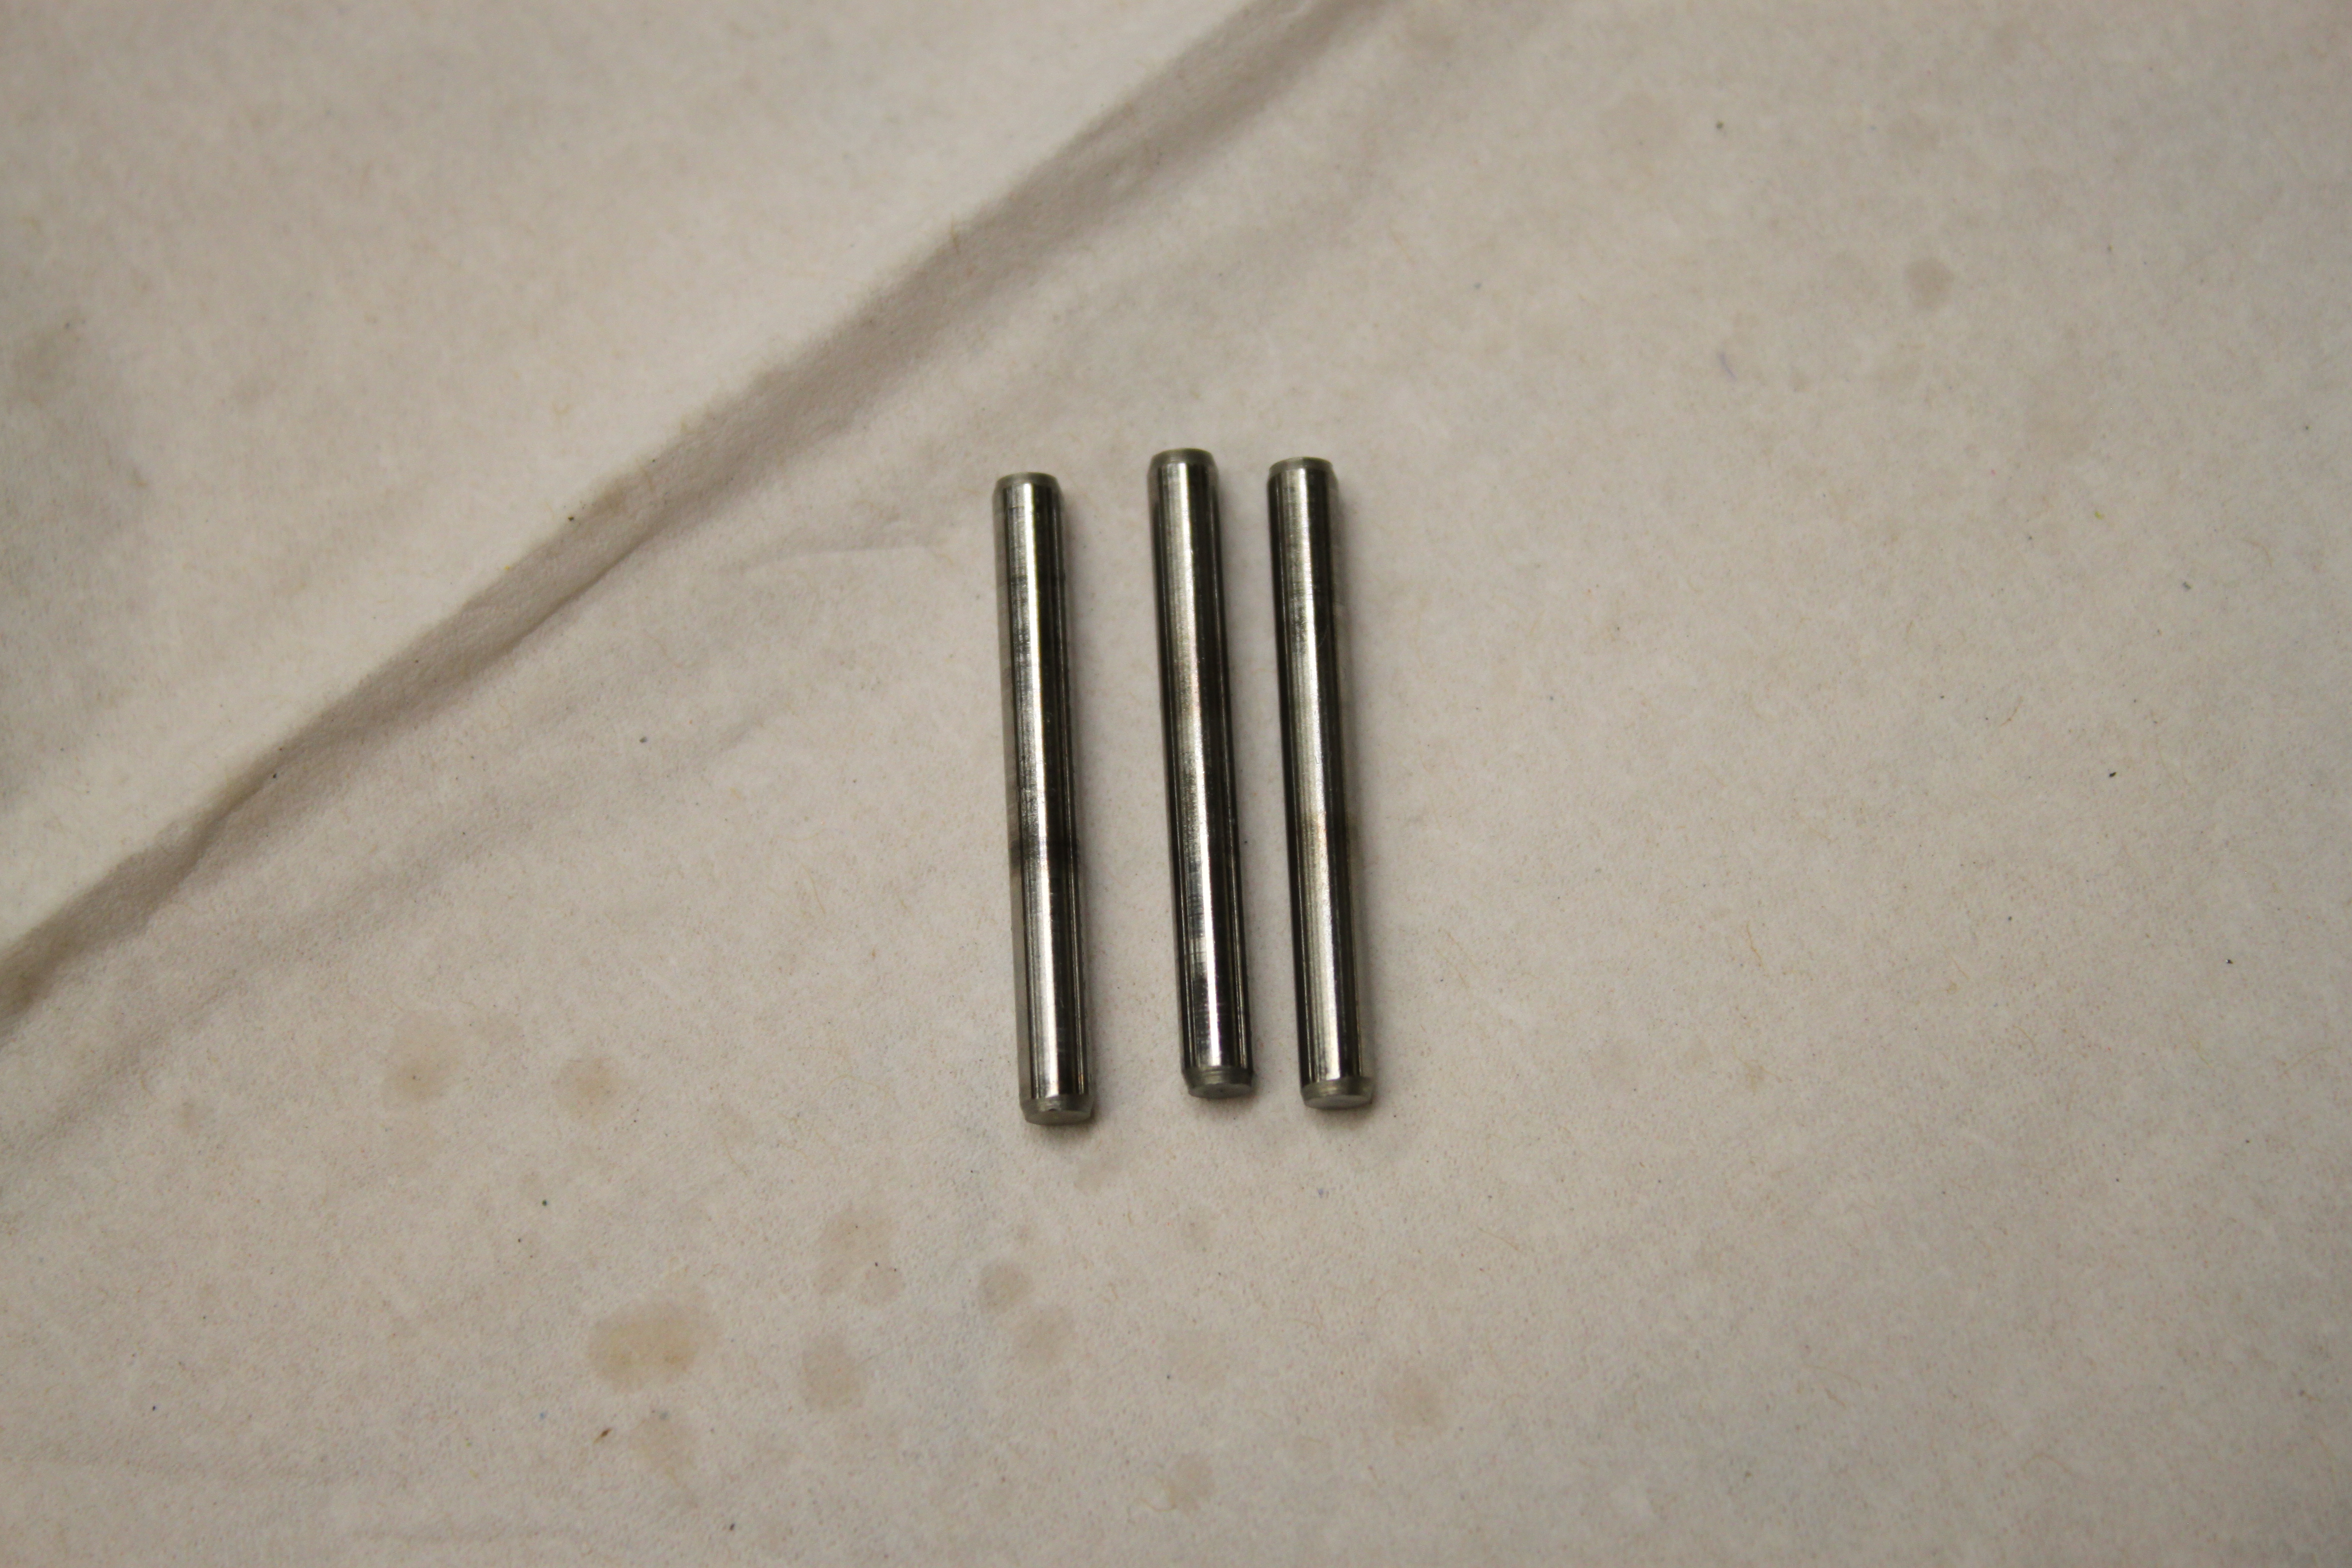
\includegraphics[width=0.3\linewidth]{fig/housing_pins}
   \caption{The pins that rest in the housing for the single-stage cycloid. The pins showed uniform wear around their diameter and across the pins, suggesting that the load was shared relatively equally around the diameter of the actuator.}
   \label{fig:single_housing_pins}
\end{figure}


The output pins can be seen in Fig \ref{fig:single_output_pins}. The output pins were fixed in the output plate and could not roll, which is evident in their wear pattern. One side of the pin has wear, while the other still has the original black oxide coating. This result makes sense since the pin is only in contact with the cycloid plate through half of the revolution. One interesting result from this though is that some pins show much more wear than others, indicating that fewer output pins were carrying load than the maximum possible, potentially resulting in more losses. A more optimal design of this system would allow these pins to roll in their housing to wear more evenly and in a potentially lower friction interaction. 

\begin{figure}[!b]
   \centering
   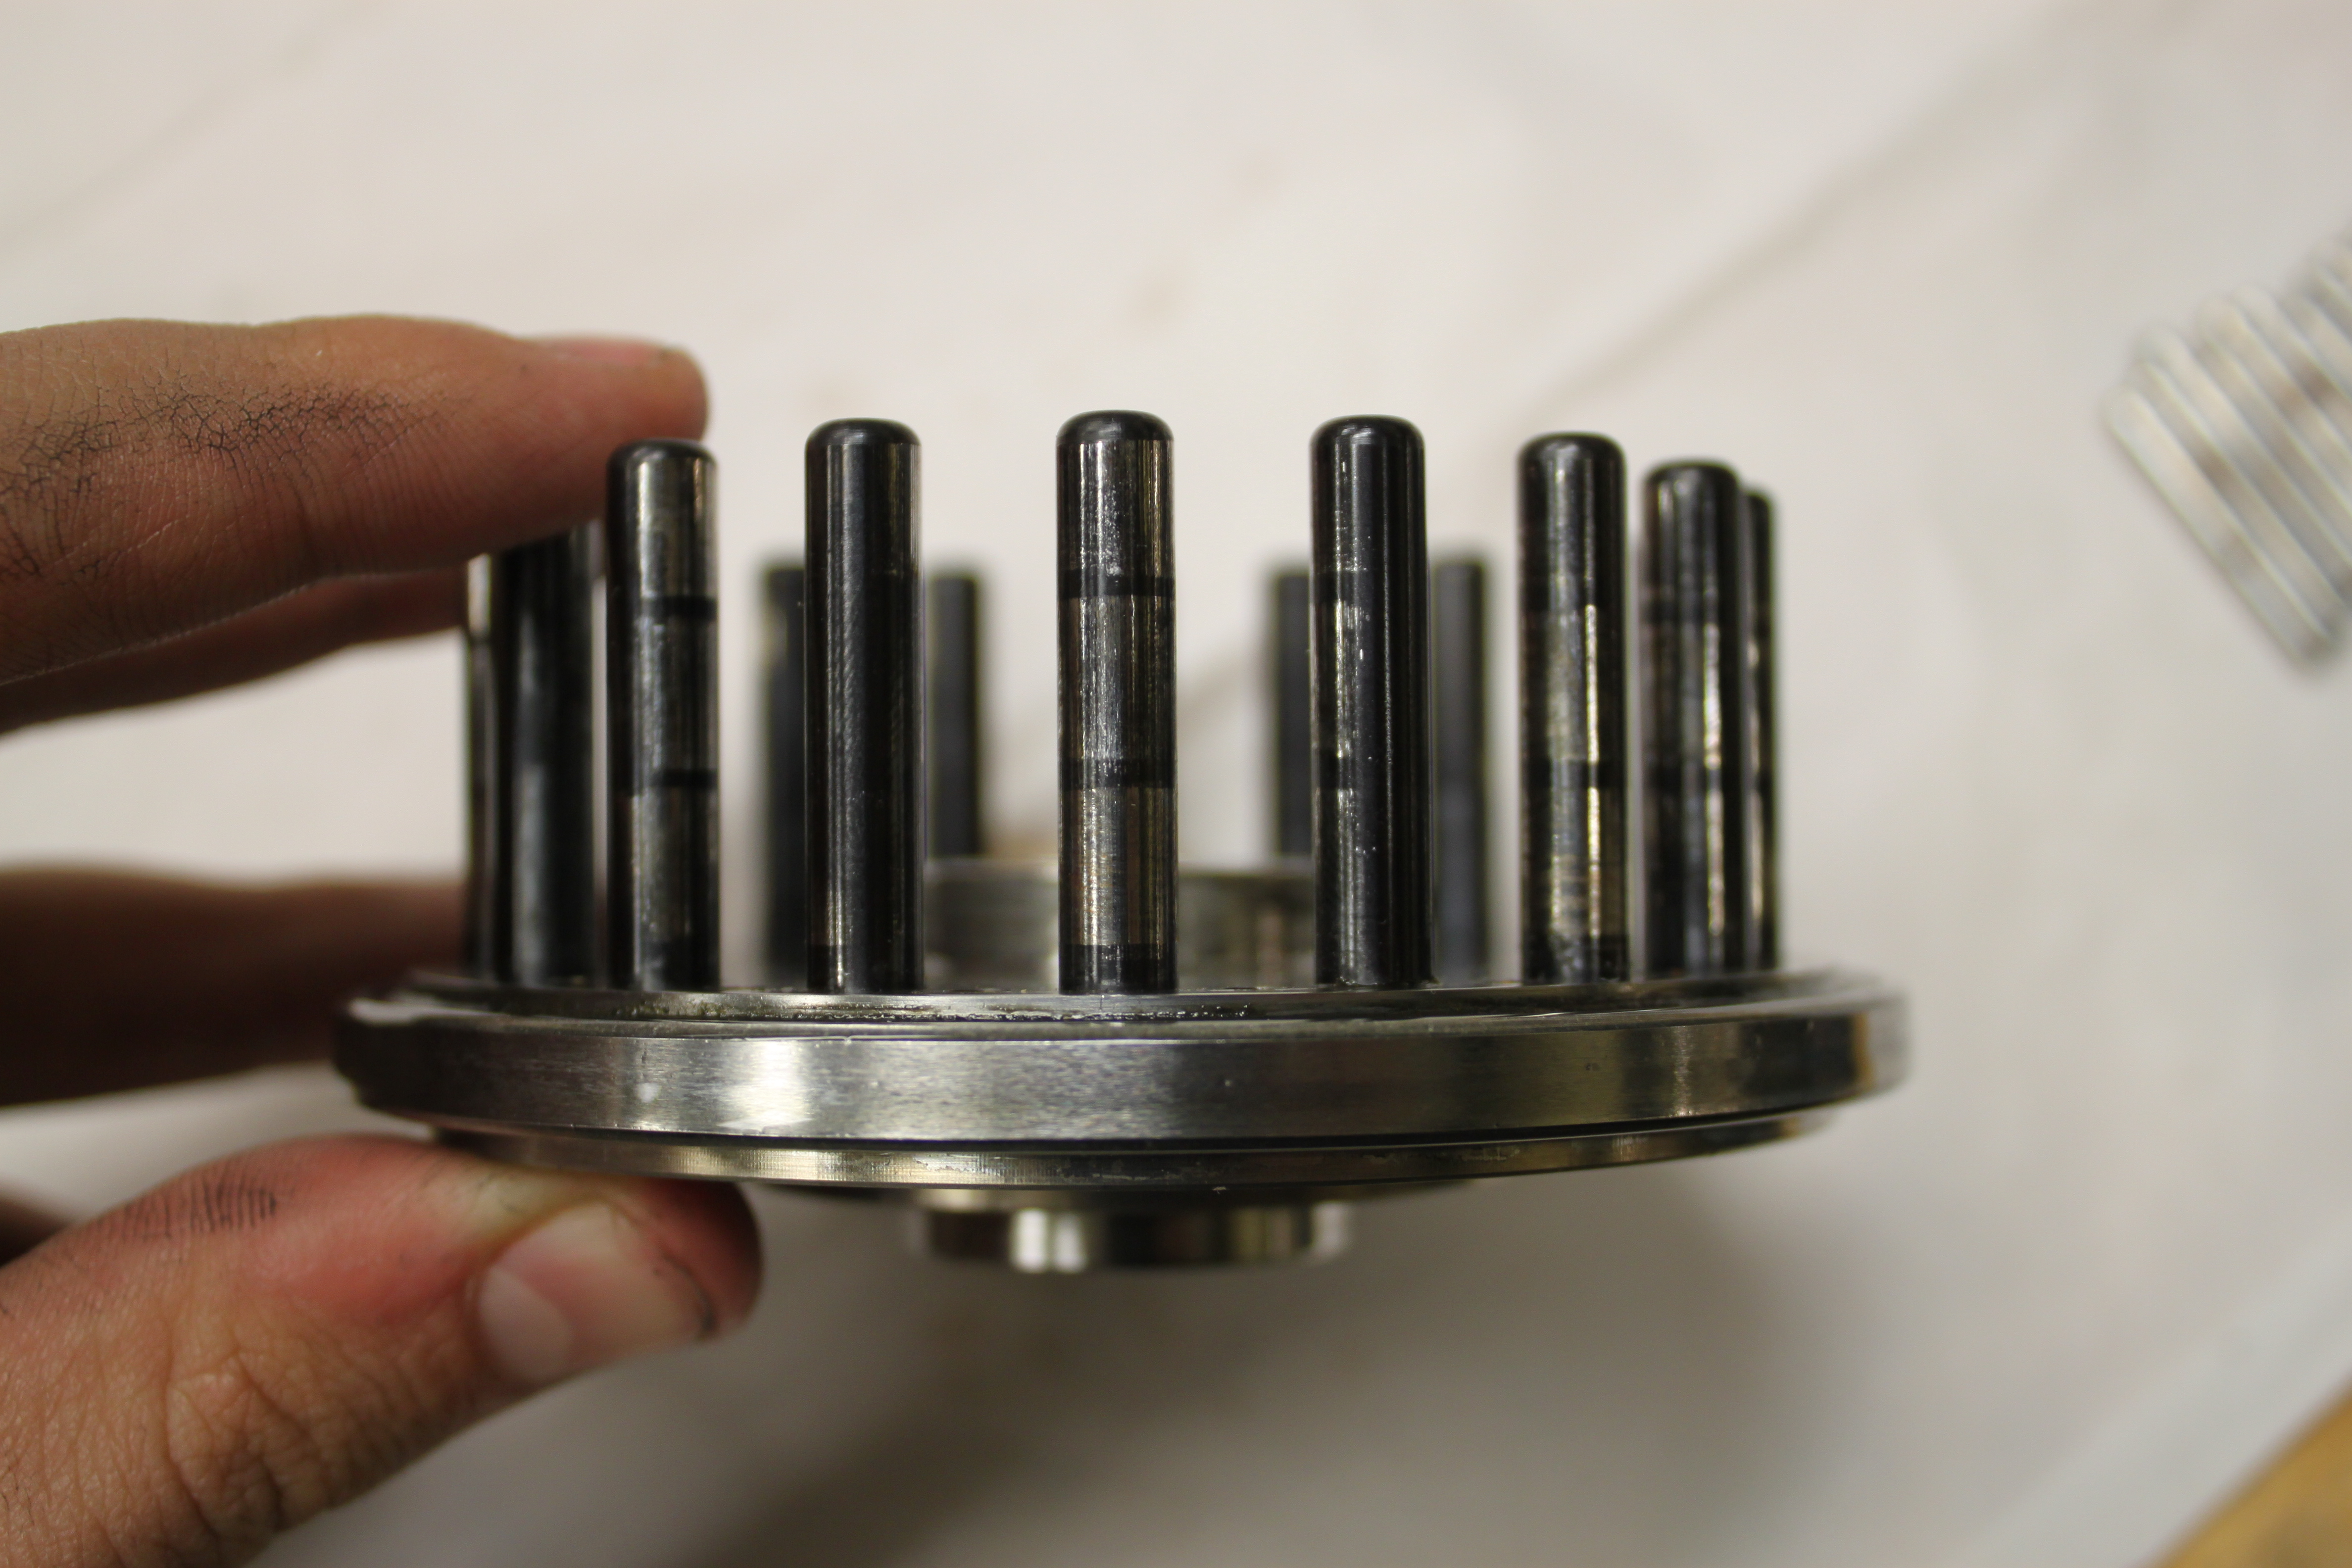
\includegraphics[width=0.7\linewidth]{fig/output_pins}
   \caption{The single-stage cycloid output pins. The pins did not rotate in their housing, so the wear is uneven around the diameter of the pin. The pins also show uneven wear from pin to pin, suggesting load was not carried equally among the pins during operation.}
   \label{fig:single_output_pins}
\end{figure}

\section{Discussion} \label{ch:single:discussion}
% Summary
% single-stage reductions built in this style can result in highly competitive efficiency ratios and 2x specific torque. You still have to deal with torque ripple and a little bit of backlash (unmeasured), but if you can handle those, drop these bad boys in. 

The efficiency of the system is dependent on the torque through the gearbox as shown in Fig \ref{fig:eff_results_final}.
This contradicts previous studies that suggested that cycloidal drives have a constant efficiency across the torque range.
There is also a much less pronounced relationship between the velocity and the cycloid efficiency that can be noted in the torque bands.
This result suggests that the cycloid efficiency behaves more like a planetary or harmonic drive gearbox in its efficiency profile.
A comparison of cycloid, harmonic, and planetary efficiency profiles can be seen in Fig \ref{fig:eff_comp}.
The figure shows the efficiency for a harmonic drive CSF-45-50-2UH-LW \cite{ref:harmonic_sheet} which has a comparable ratio and torque capability to the tested cycloid and weighs 5.1kg, and a representative planetary efficiency curve from the engineers at Maxon Motor.
If backlash is acceptable in a system, a cycloidal drive can provide similar or better efficiency profiles to a harmonic drive while providing a potential 2x increase in specific torque (Nm/kg).

\begin{figure}[h]
   \centering
   \includegraphics[width=0.7\linewidth]{fig/eff_comp_v3}
   \caption{Comparison of efficiency over maximum torque rating of the tested cycloid, a comparable harmonic drive, and a theoretical planetary gearset.
   The cycloid exhibits the same efficiency increase over torque range and has a comparable and slightly higher efficiency than the harmonic.}
   \label{fig:eff_comp}
\end{figure}

\begin{figure}[h]
   \centering
   \includegraphics[width=\linewidth]{fig/burn_in}
   \caption{The first three days of testing show a substantial wear-in period for high torque periods.}
   \label{fig:break_in}
\end{figure}
\todo[inline]{fix legend size}

There was a substantial break-in time for the actuator before steady state results were achieved highlighted in Fig \ref{fig:break_in}).
In the high torque case, specifically in the reverse direction, there was an approximately linear increase in efficiency over the course of the first seven hours of duty cycle testing.
This testing began after a minimum of five hours of run time spread out through many short sessions while getting the test system running.
The large increase in efficiency can be noted in the other lower torque profiles as well, starting well below their final steady state values.
The authors theorize that this is due to break-in of the manufactured parts required because of machining inaccuracies.
Due to the complex interaction required of the trochoidal motion profile, slight manufacturing deficiencies could cause build-ups of stress and loss in particular points on the drive.
It would make sense that these could manifest in one direction and not the other if a lobe was misshapen on the trailing edge in one direction, it would be the lead in the other, causing the additional loss.
Through the first hours of testing, these materials likely wore in to each other until the contact was smooth, resulting in the more readily achieved steady state efficiencies in subsequent hours of testing.

Additionally, there is a marked improvement over the first 30 minutes of runtime in the efficiency of the system.
This is likely due to the grease and heat in the system.
The gearbox is greased with Lucas Oil Red'N'Tacky which has a viscosity index of 86 min.
This was chosen because it is designed for high loads for extended periods of time in gear and sliding surface applications, as well as ease of use for Earth testing and verification.
Therefore, during the warm-up period as the actuator temperature increases, the viscosity decrease is likely enough to cause a notable increase in efficiency of the system.
The authors leave the study of a lower viscosity grease's effect on performance, as well as grease suitable for vacuum, for future work.

Finally, through the efficiency comparison after 100 hours of testing (Fig. \ref{fig:eff_results}) and 300 hours of testing (Fig. \ref{fig:eff_results_final}) there was no appreciable loss in efficiency of the system. The actuator maintained a high level of efficiency, 81\% peak, throughout the testing. This result, coupled with the qualitative analysis of the parts after disassembly suggests that the lifetime of this actuator can greatly exceed the current testing of 129k revolutions, which suggests this is a viable actuator for robotic systems where backlash is acceptable and a high reduction and high torque actuator is necessary. 



%!TEX root = thesis_main.tex

\chapter{Testing and Analysis of Dual Stage Cycloid}\label{ch:dual}


\section{Test Setup} \label{dual:test_setupd}

typity type type type
new line

double new line 

\section{Results} \label{dual:results}

\section{Discussion} \label{dual:discussion}

%!TEX root = thesis_main.tex

\chapter{Conclusion}\label{ch:conclusion}
% I did it I did it... Now give me my piece of paper! 





\appendix
\include{appendix-a}

\bibliographystyle{ieeetr}
\bibliography{thesisBib}
\end{document}
